\section{MINERAL RESOURCES (2nd floor)}

The second floor of the Ho Chi Minh City Geological Museum showcases Vietnam's abundant mineral wealth and geological resources. This floor provides comprehensive displays of various mineral categories, from energy resources to precious gemstones, offering visitors insight into the country's geological diversity and economic potential. The exhibits demonstrate how these natural resources have been formed through millions of years of geological processes and their significance to Vietnam's development.

\subsection{Energy and Fuel Resources}

Energy resources represent naturally occurring materials that can be utilized to generate power and heat through combustion or other processes. The museum's collection highlights two fundamental categories of fossil fuels that have shaped Vietnam's energy landscape.

\textbf{Petroleum} constitutes a crucial liquid hydrocarbon resource formed from ancient marine organisms subjected to heat and pressure over geological time scales. This valuable resource undergoes refining processes to produce essential fuels including gasoline, diesel fuel, and aviation kerosene. Vietnam's petroleum reserves, particularly in offshore basins, play a vital role in the nation's energy security and economic development.

\begin{figure}[H]
\centering
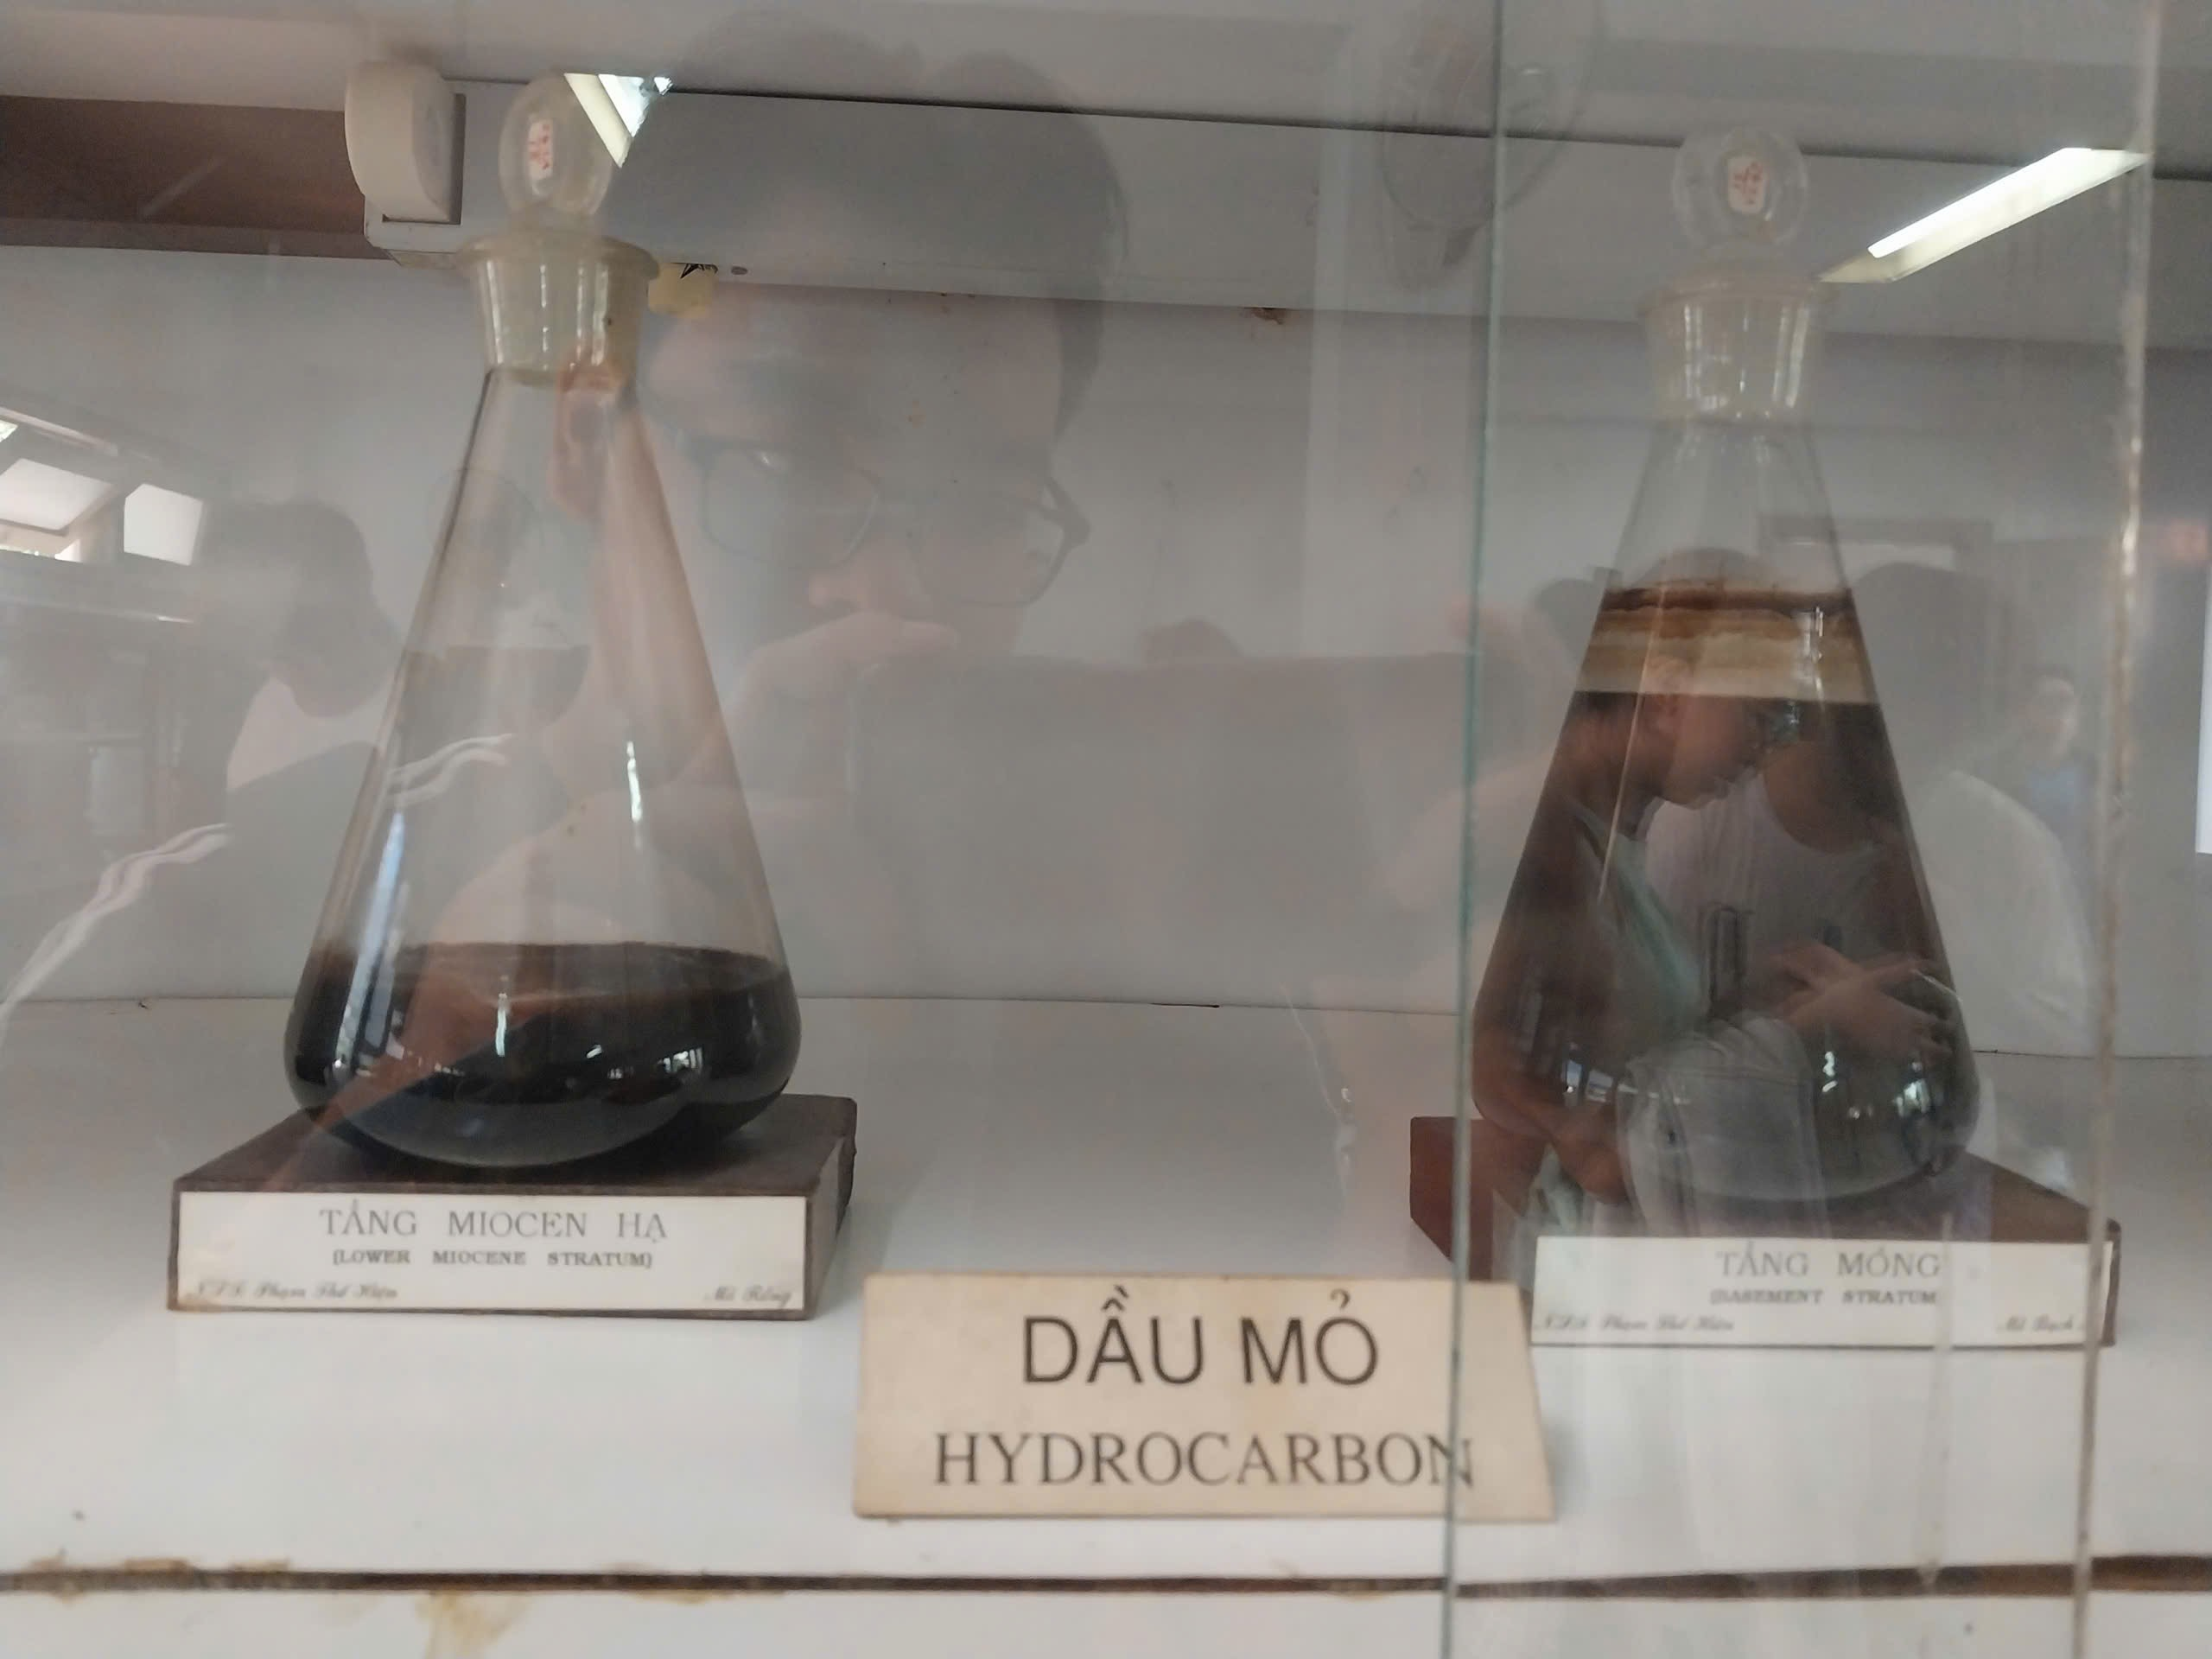
\includegraphics[width=0.7\textwidth]{graphics/petroleum_sample.png}
\caption{Petroleum sample display from Vietnamese offshore reserves}
\label{fig:petroleum}
\end{figure}

\textbf{Coal} represents a solid fossil fuel derived from ancient plant matter that underwent transformation through geological compression and heating over millions of years. The museum displays various coal types classified by their carbon content and energy density:
\begin{itemize}
    \item Peat -- representing the earliest stage of coal development
    \item Lignite -- commonly referred to as brown coal with moderate energy content
    \item Bituminous coal -- a widely utilized intermediate-grade coal
    \item Anthracite -- the highest quality coal with maximum energy output
\end{itemize}

\begin{figure}[H]
\centering
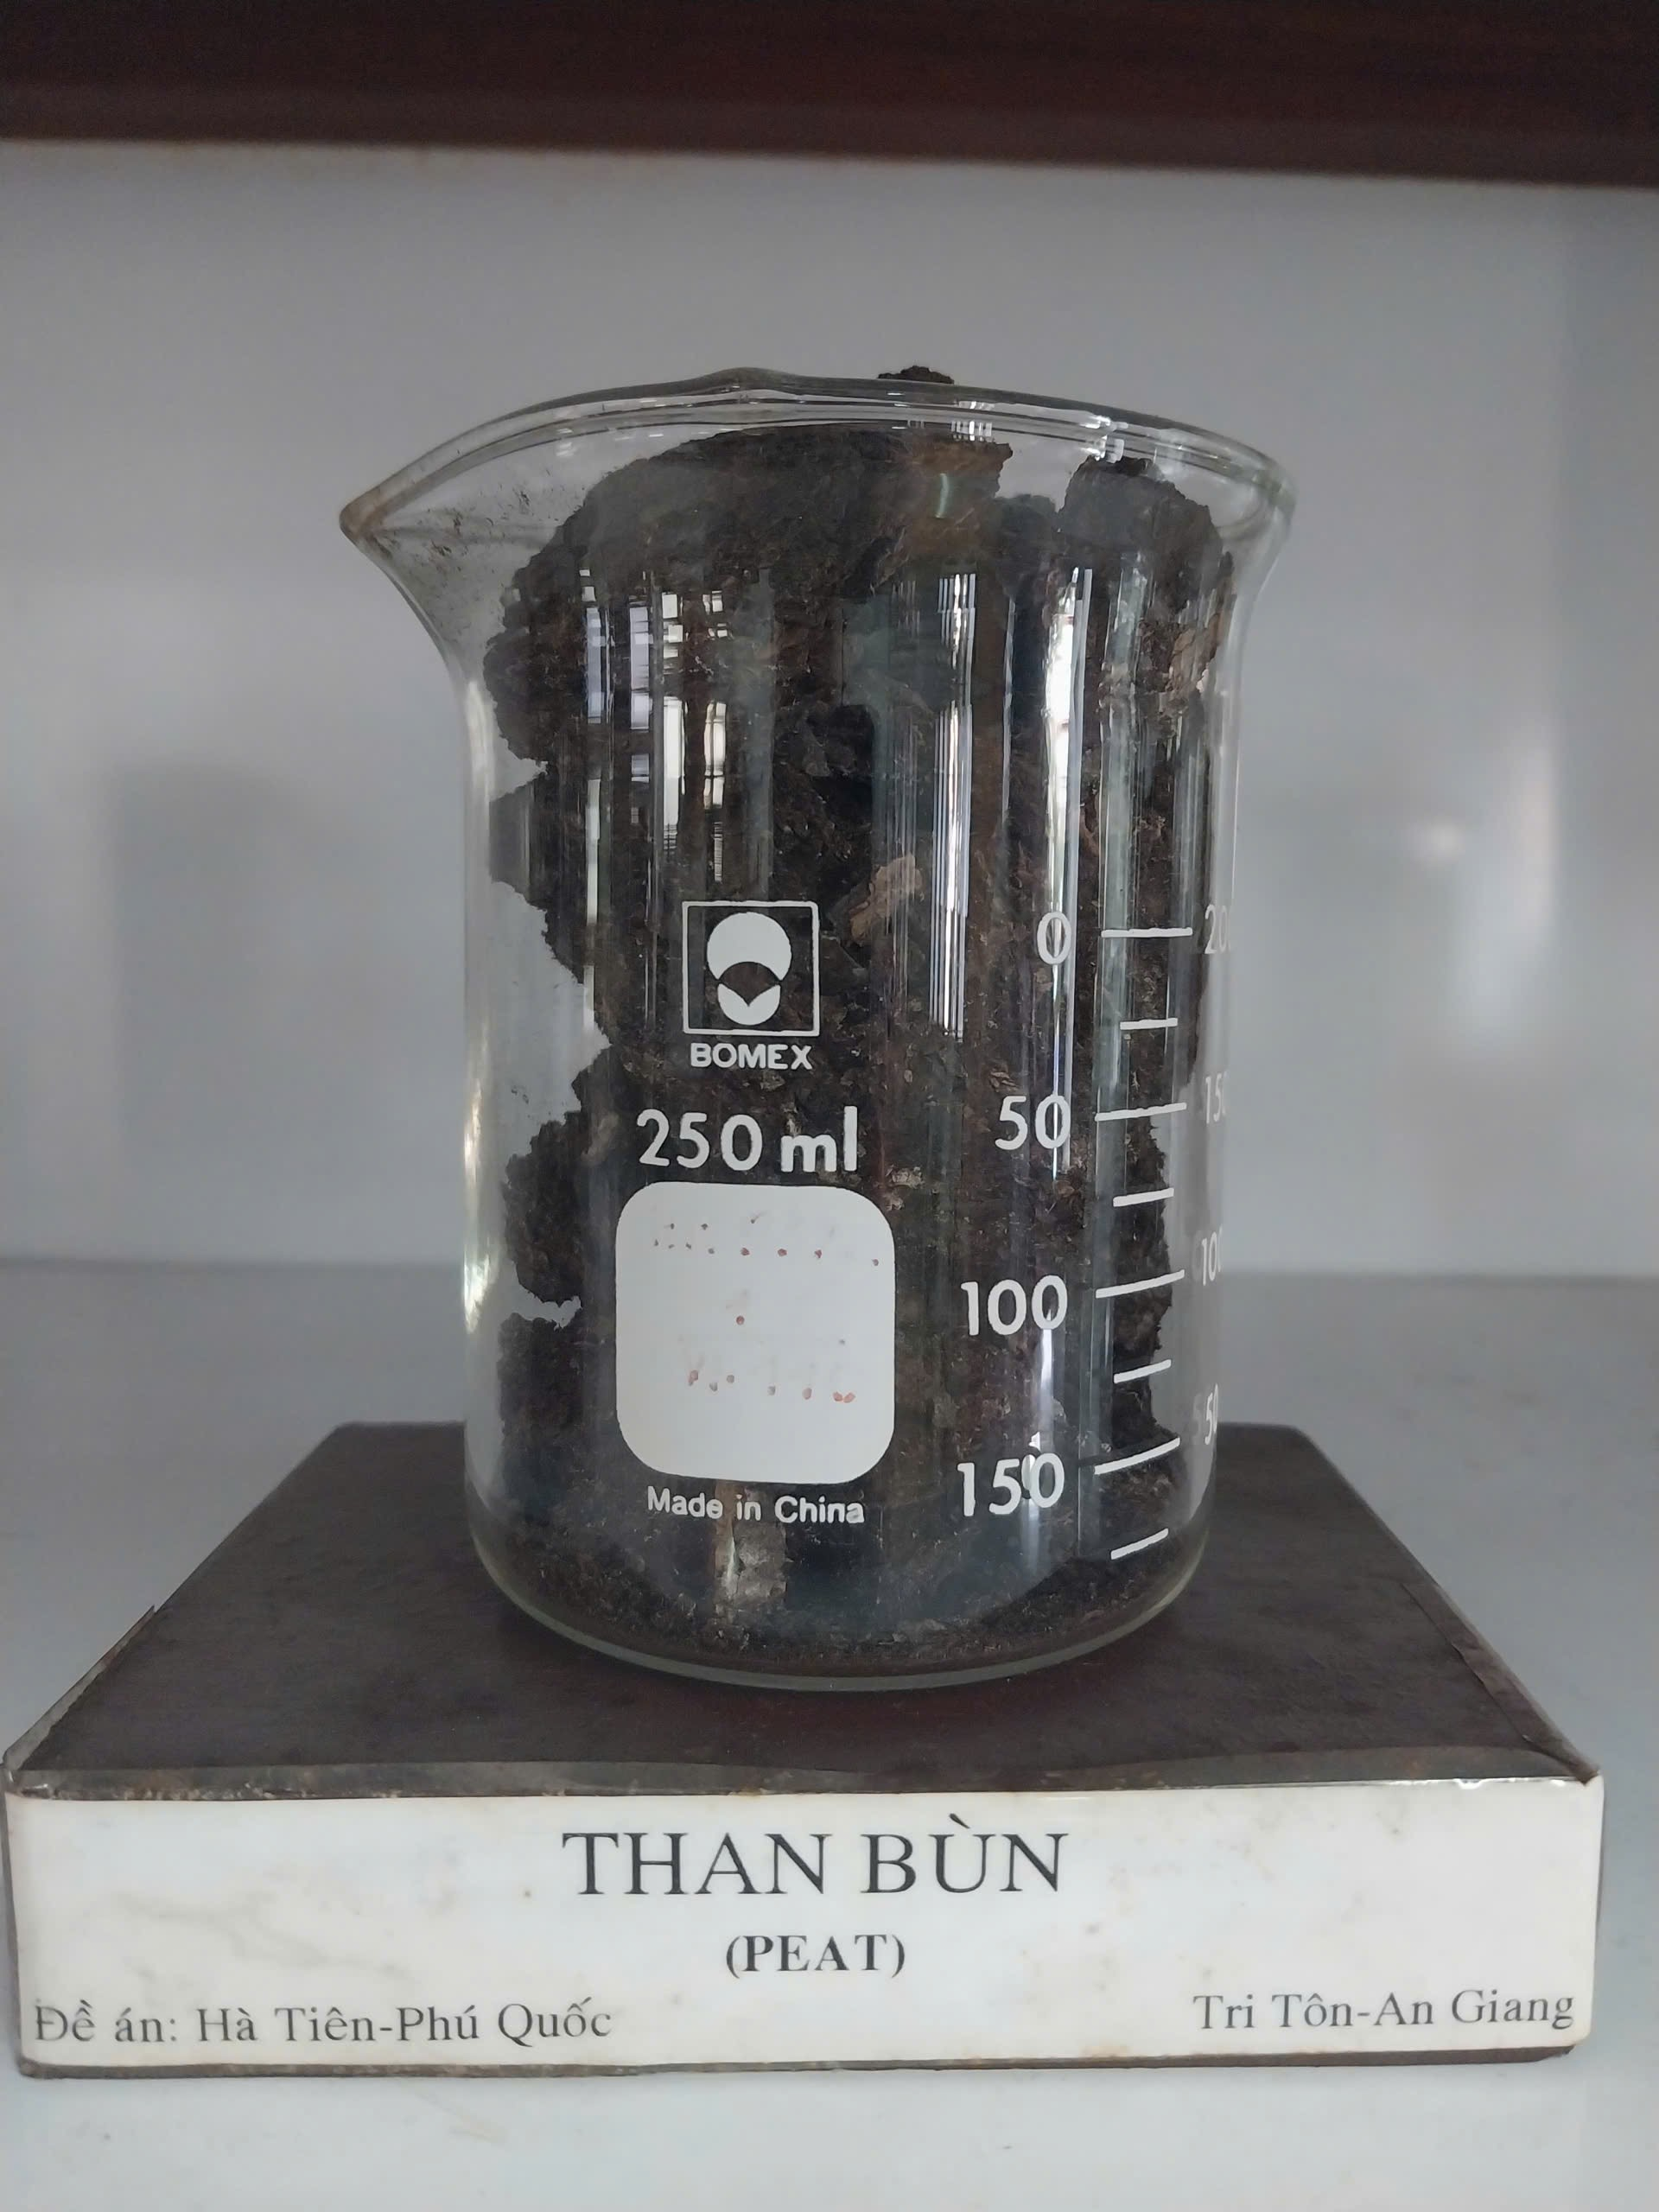
\includegraphics[width=0.7\textwidth]{graphics/coal_types.png}
\caption{Different types of coal samples showing progression from peat to anthracite}
\label{fig:coal_types}
\end{figure}

These coal varieties serve primarily in electrical power generation and industrial applications, including steel production processes.

\begin{figure}[H]
\centering
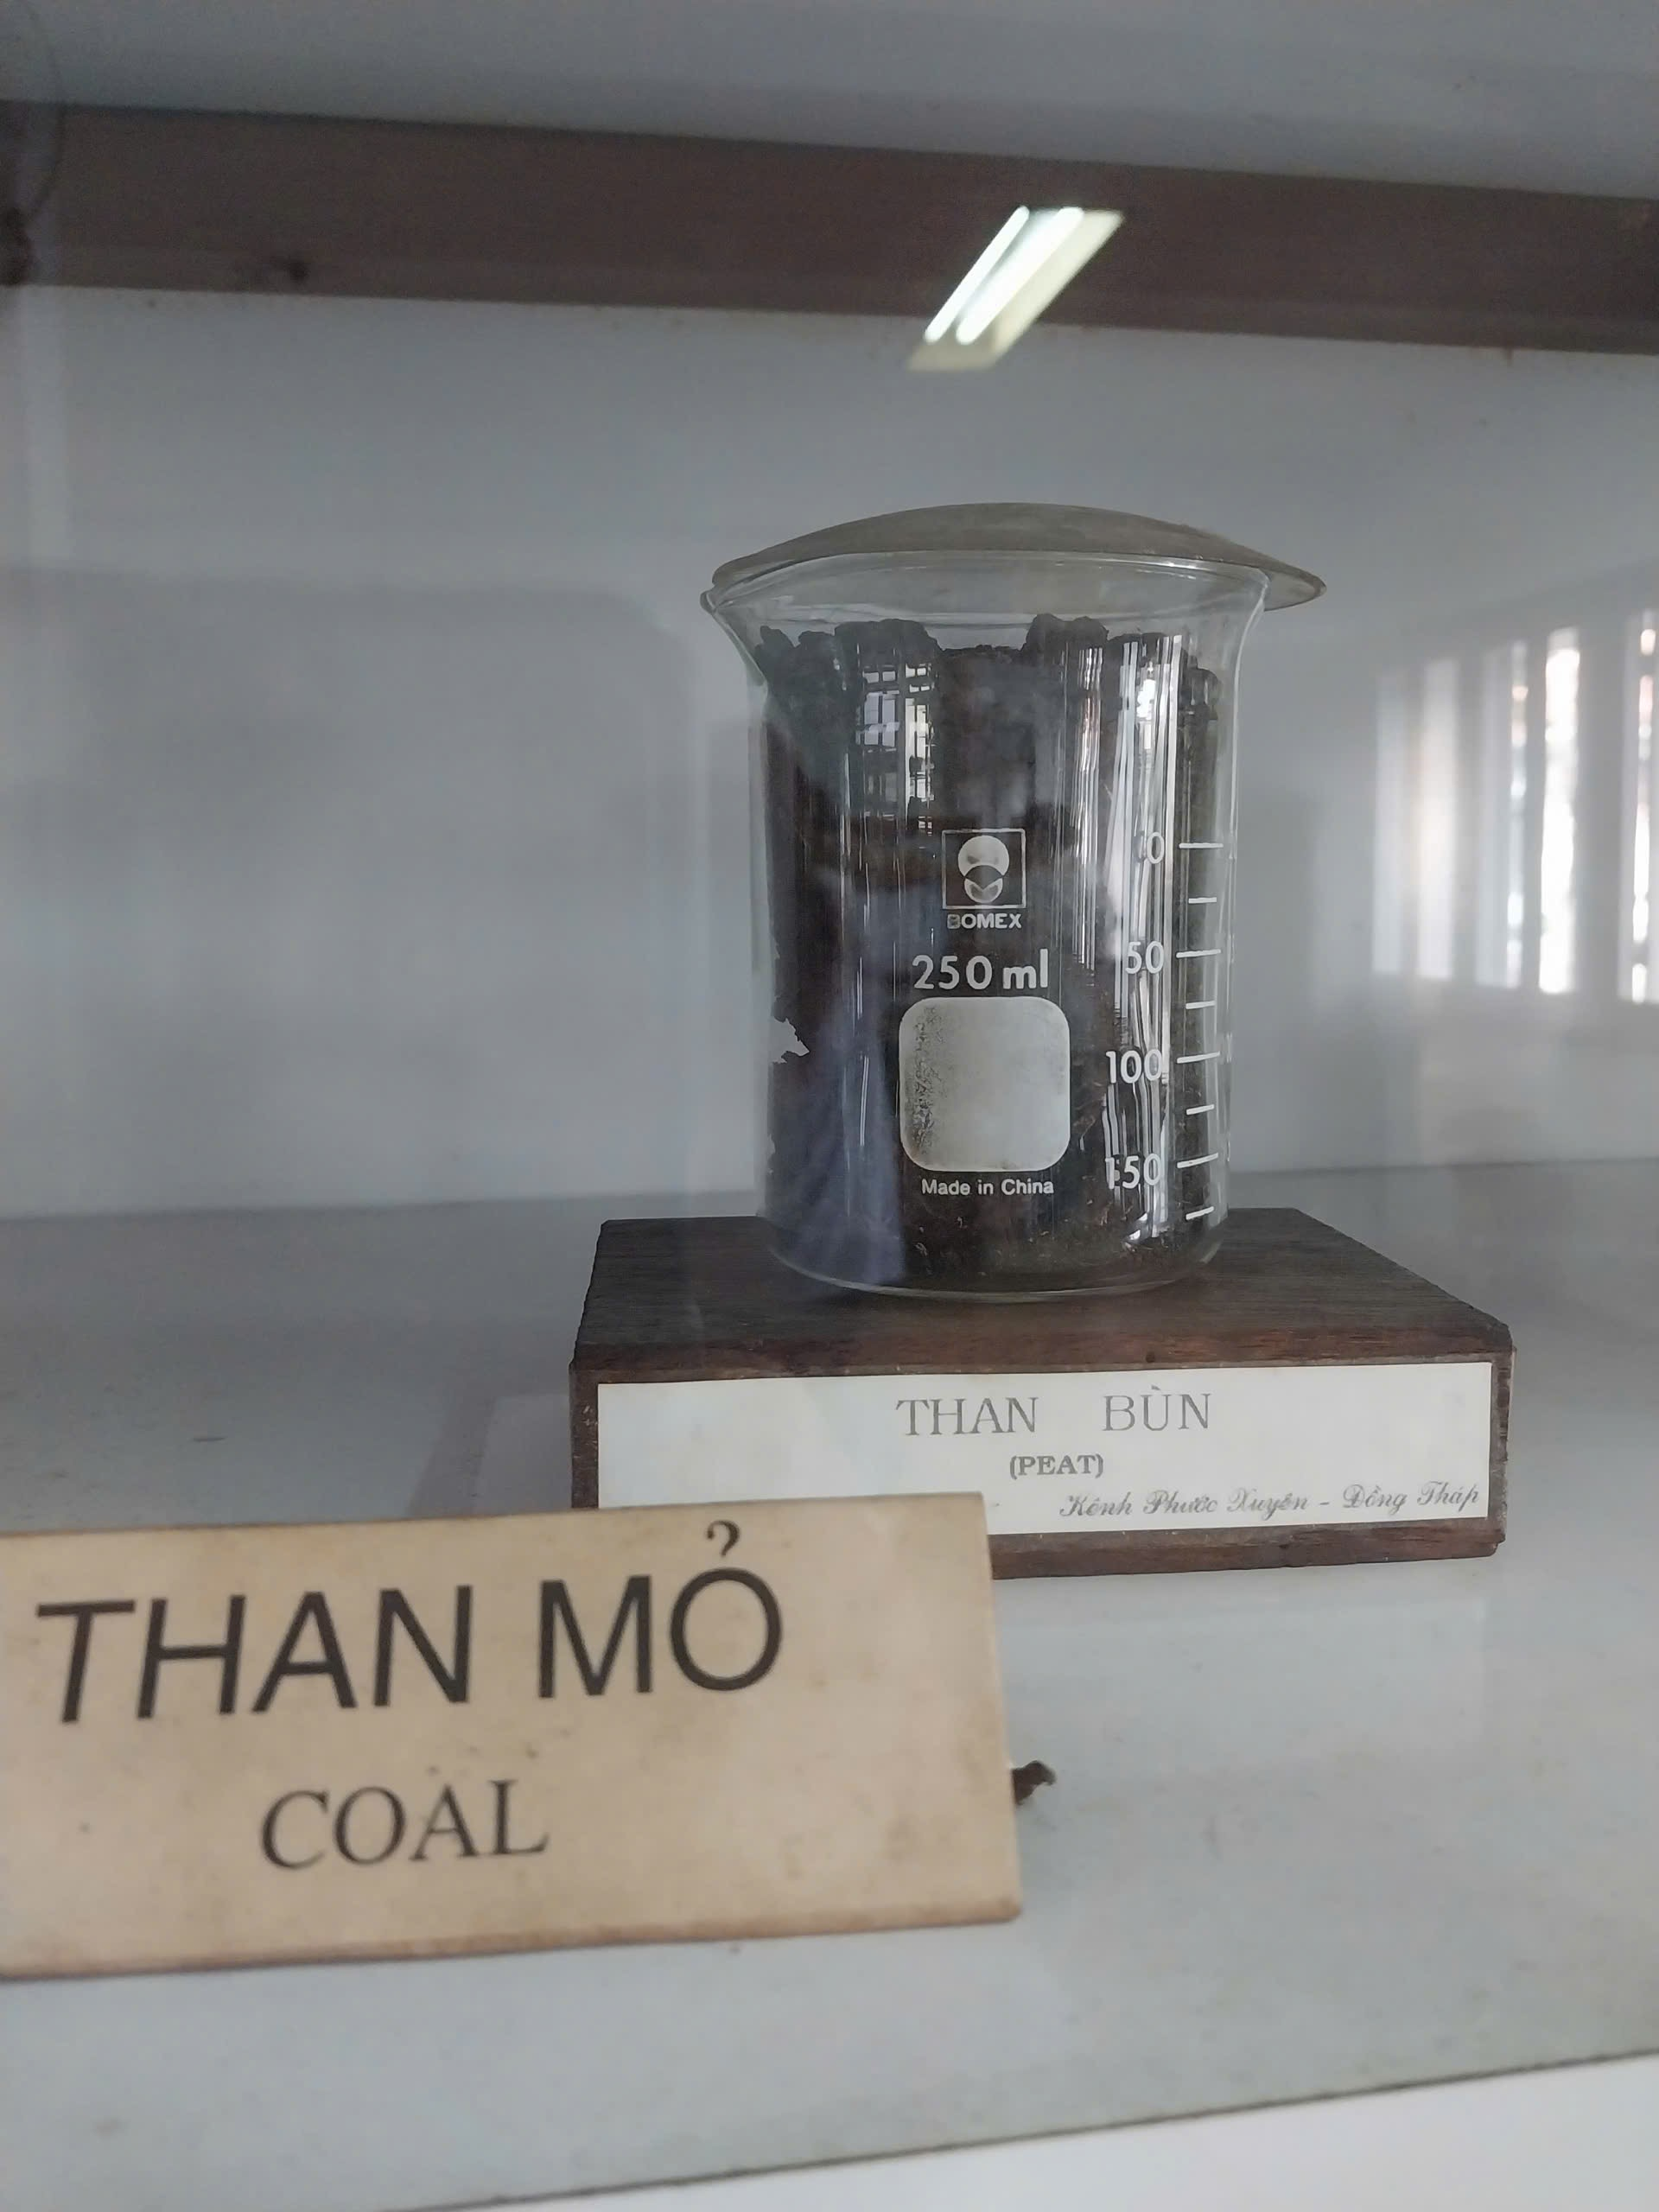
\includegraphics[width=0.7\textwidth]{graphics/coal_types_2.png}
\caption{Additional coal specimens from Vietnamese geological formations}
\label{fig:coal_specimens}
\end{figure}

\subsection{Metallic Mineral Resources}

Vietnam possesses diverse metallic mineral resources distributed across different geological regions.

\textbf{Strategic Metals}
\textit{Titanium:} A lightweight, strong, and corrosion-resistant metal used in aerospace and medical applications. Vietnam has titanium deposits primarily in coastal sand formations.

\textit{Tin:} Vietnam is one of the world's significant tin producers, with major deposits in the northern provinces. Tin is essential for electronics and soldering applications.

\textit{Chromium:} Used in stainless steel production and chrome plating. Vietnam's chromium deposits are found in ultramafic rock formations.

\textit{Rare Earth Elements:} Critical for modern technology including electronics, renewable energy systems, and defense applications.

\begin{figure}[H]
\centering
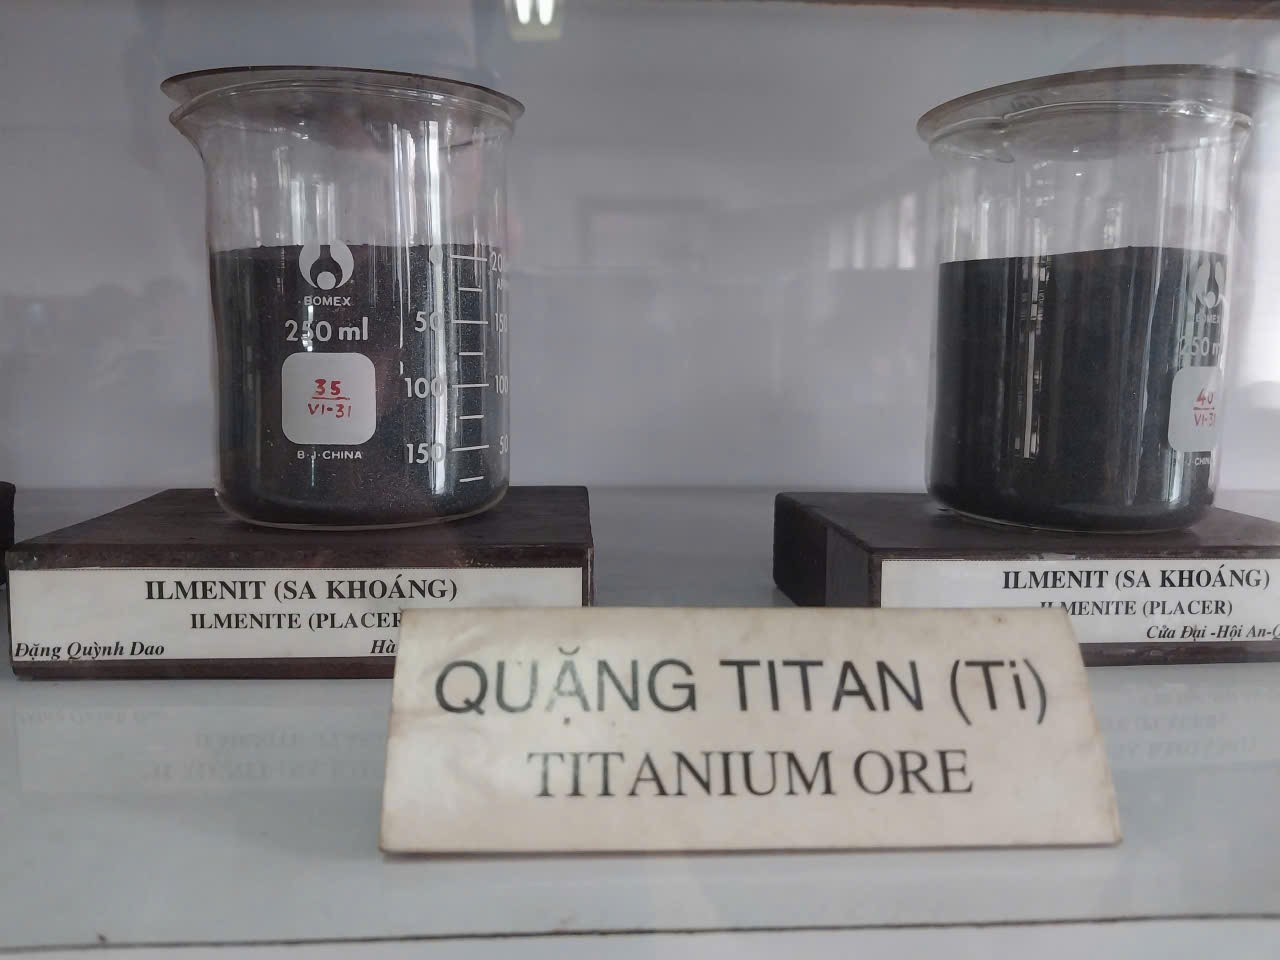
\includegraphics[width=0.7\textwidth]{graphics/strategic_metals.png}
\caption{Strategic metal samples including titanium and rare earth elements}
\label{fig:strategic_metals}
\end{figure}

\textbf{Industrial Metals}
\textit{Iron:} The foundation of steel production, Vietnam has significant iron ore deposits in the northern regions, particularly in Thai Nguyen and Lao Cai provinces.

\textit{Aluminum:} Derived from bauxite ore, Vietnam has substantial bauxite reserves in the Central Highlands region.

\textit{Copper:} Essential for electrical applications and construction. Vietnam's copper deposits are found in various geological formations.

\textit{Zinc:} Used in galvanizing and alloy production. Vietnam has zinc deposits associated with lead mineralization.

\textit{Lead:} Important for batteries and radiation shielding applications.

\begin{figure}[H]
\centering
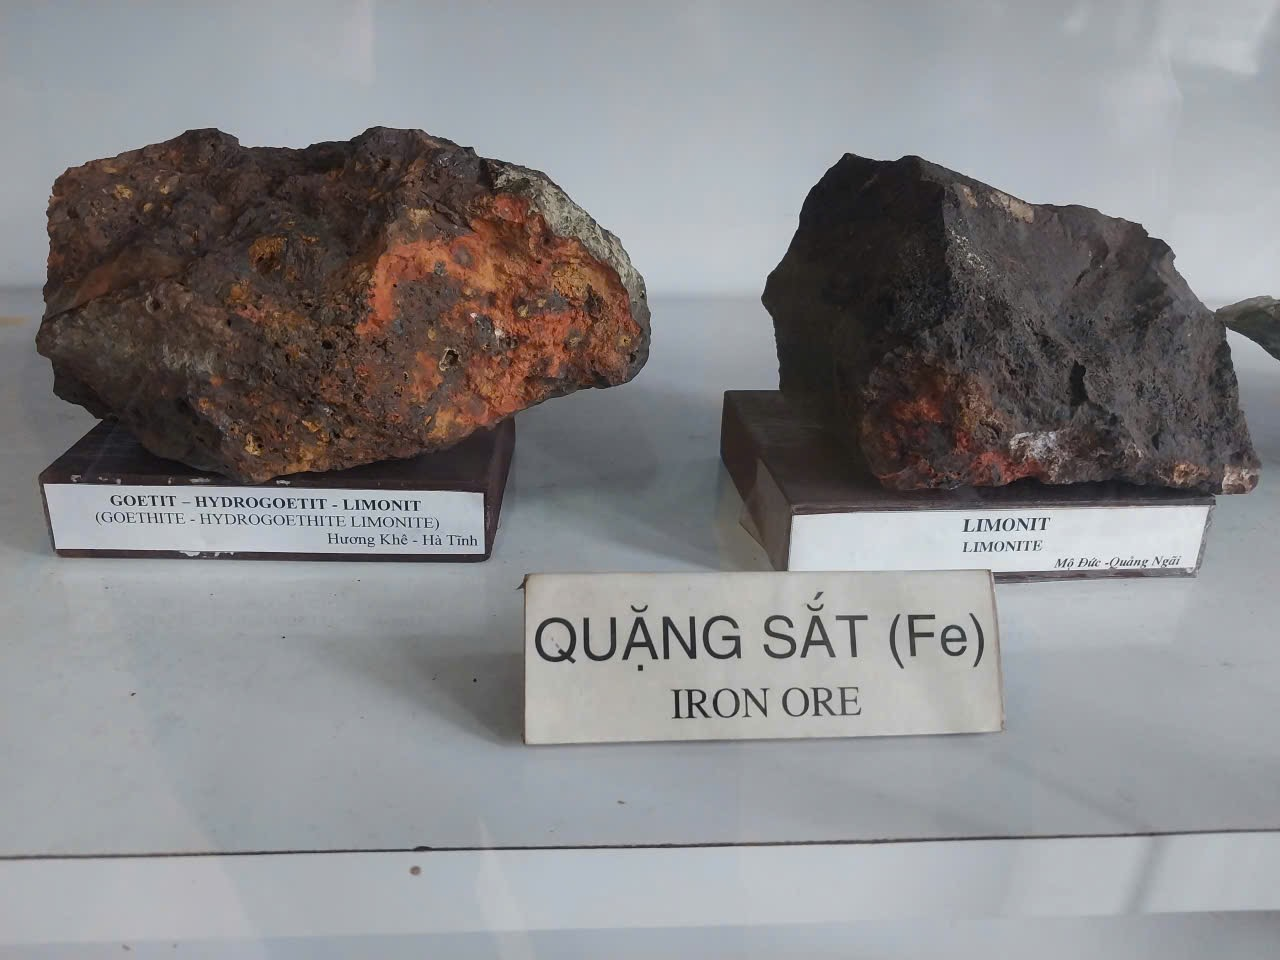
\includegraphics[width=0.7\textwidth]{graphics/industrial_metals.png}
\caption{Industrial metal samples including iron ore and copper}
\label{fig:industrial_metals}
\end{figure}

\textbf{Precious Metals}
\textit{Gold:} Vietnam has both placer and lode gold deposits. Gold mining has a long history in Vietnam, with significant deposits in Quang Nam and other provinces.

\textit{Silver:} Often found associated with other metal ores, silver has both monetary and industrial applications.

\begin{figure}[H]
\centering
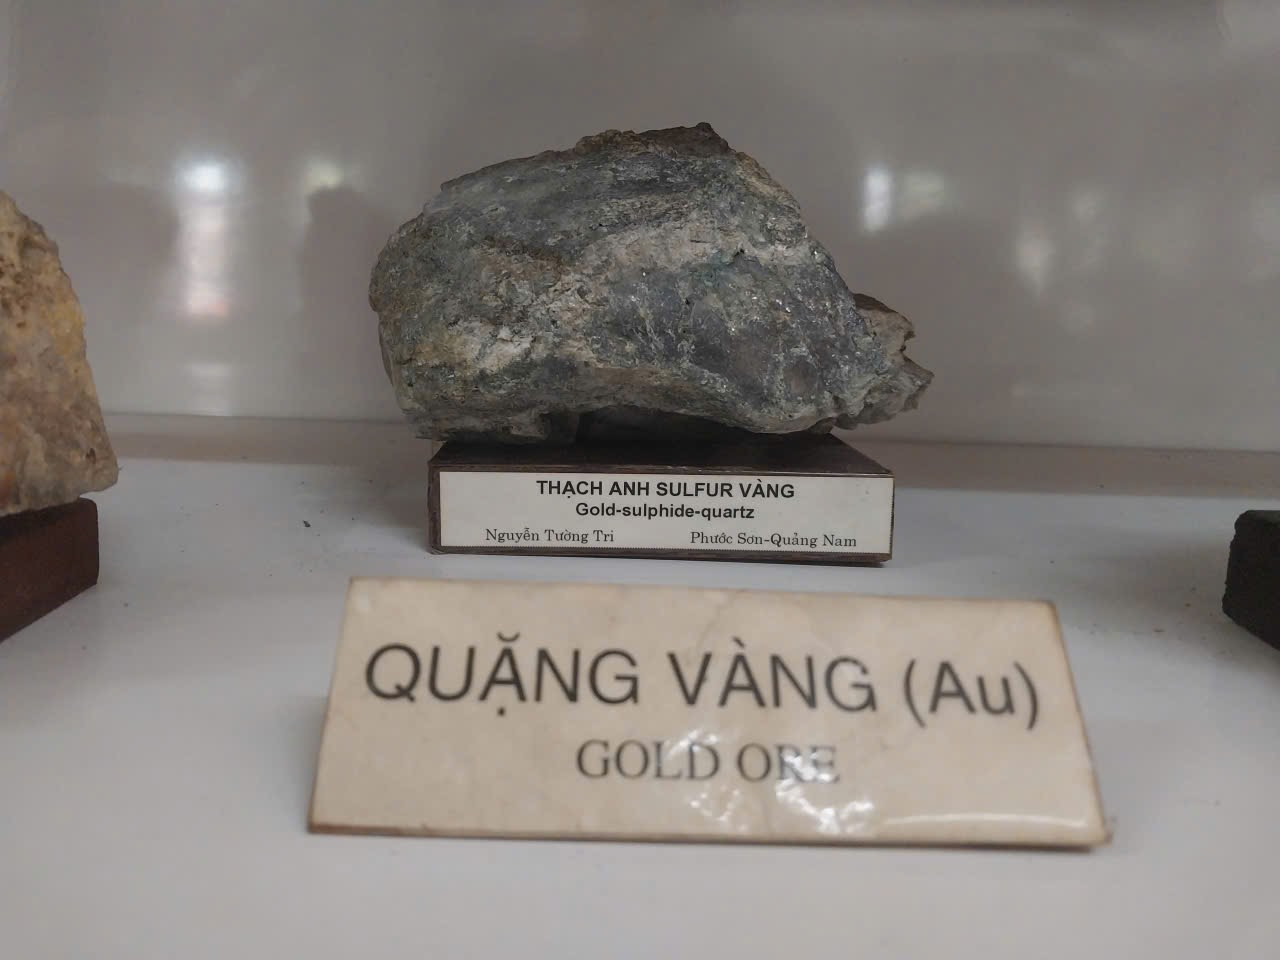
\includegraphics[width=0.7\textwidth]{graphics/precious_metals.png}
\caption{Gold and silver samples from Vietnamese deposits}
\label{fig:precious_metals}
\end{figure}

\textbf{Specialty Metals}
\textit{Tungsten:} Vietnam is a major tungsten producer globally. Tungsten is essential for high-temperature applications and cutting tools.

\textit{Molybdenum:} Used in steel alloys and high-temperature applications.

\textit{Magnesium:} Lightweight metal used in aerospace and automotive industries.

\subsection{Non-Metallic Mineral Resources}

Non-metallic minerals represent naturally occurring substances lacking metallic properties but possessing significant industrial and economic value. These materials serve essential functions in construction, agriculture, and manufacturing sectors.

\textbf{Industrial Minerals}
\textit{Silica Sand:} High-purity silica sand is essential for glass manufacturing, foundry operations, and construction applications. Vietnam has significant silica sand deposits along its coastal regions, particularly suitable for high-quality glass production.

\textit{Pyrite:} Iron sulfide mineral (\ce{FeS2}) with applications in sulfuric acid production and as a source of sulfur for chemical industries. Pyrite is also known as "fool's gold" due to its metallic luster and golden color.

\begin{figure}[H]
\centering
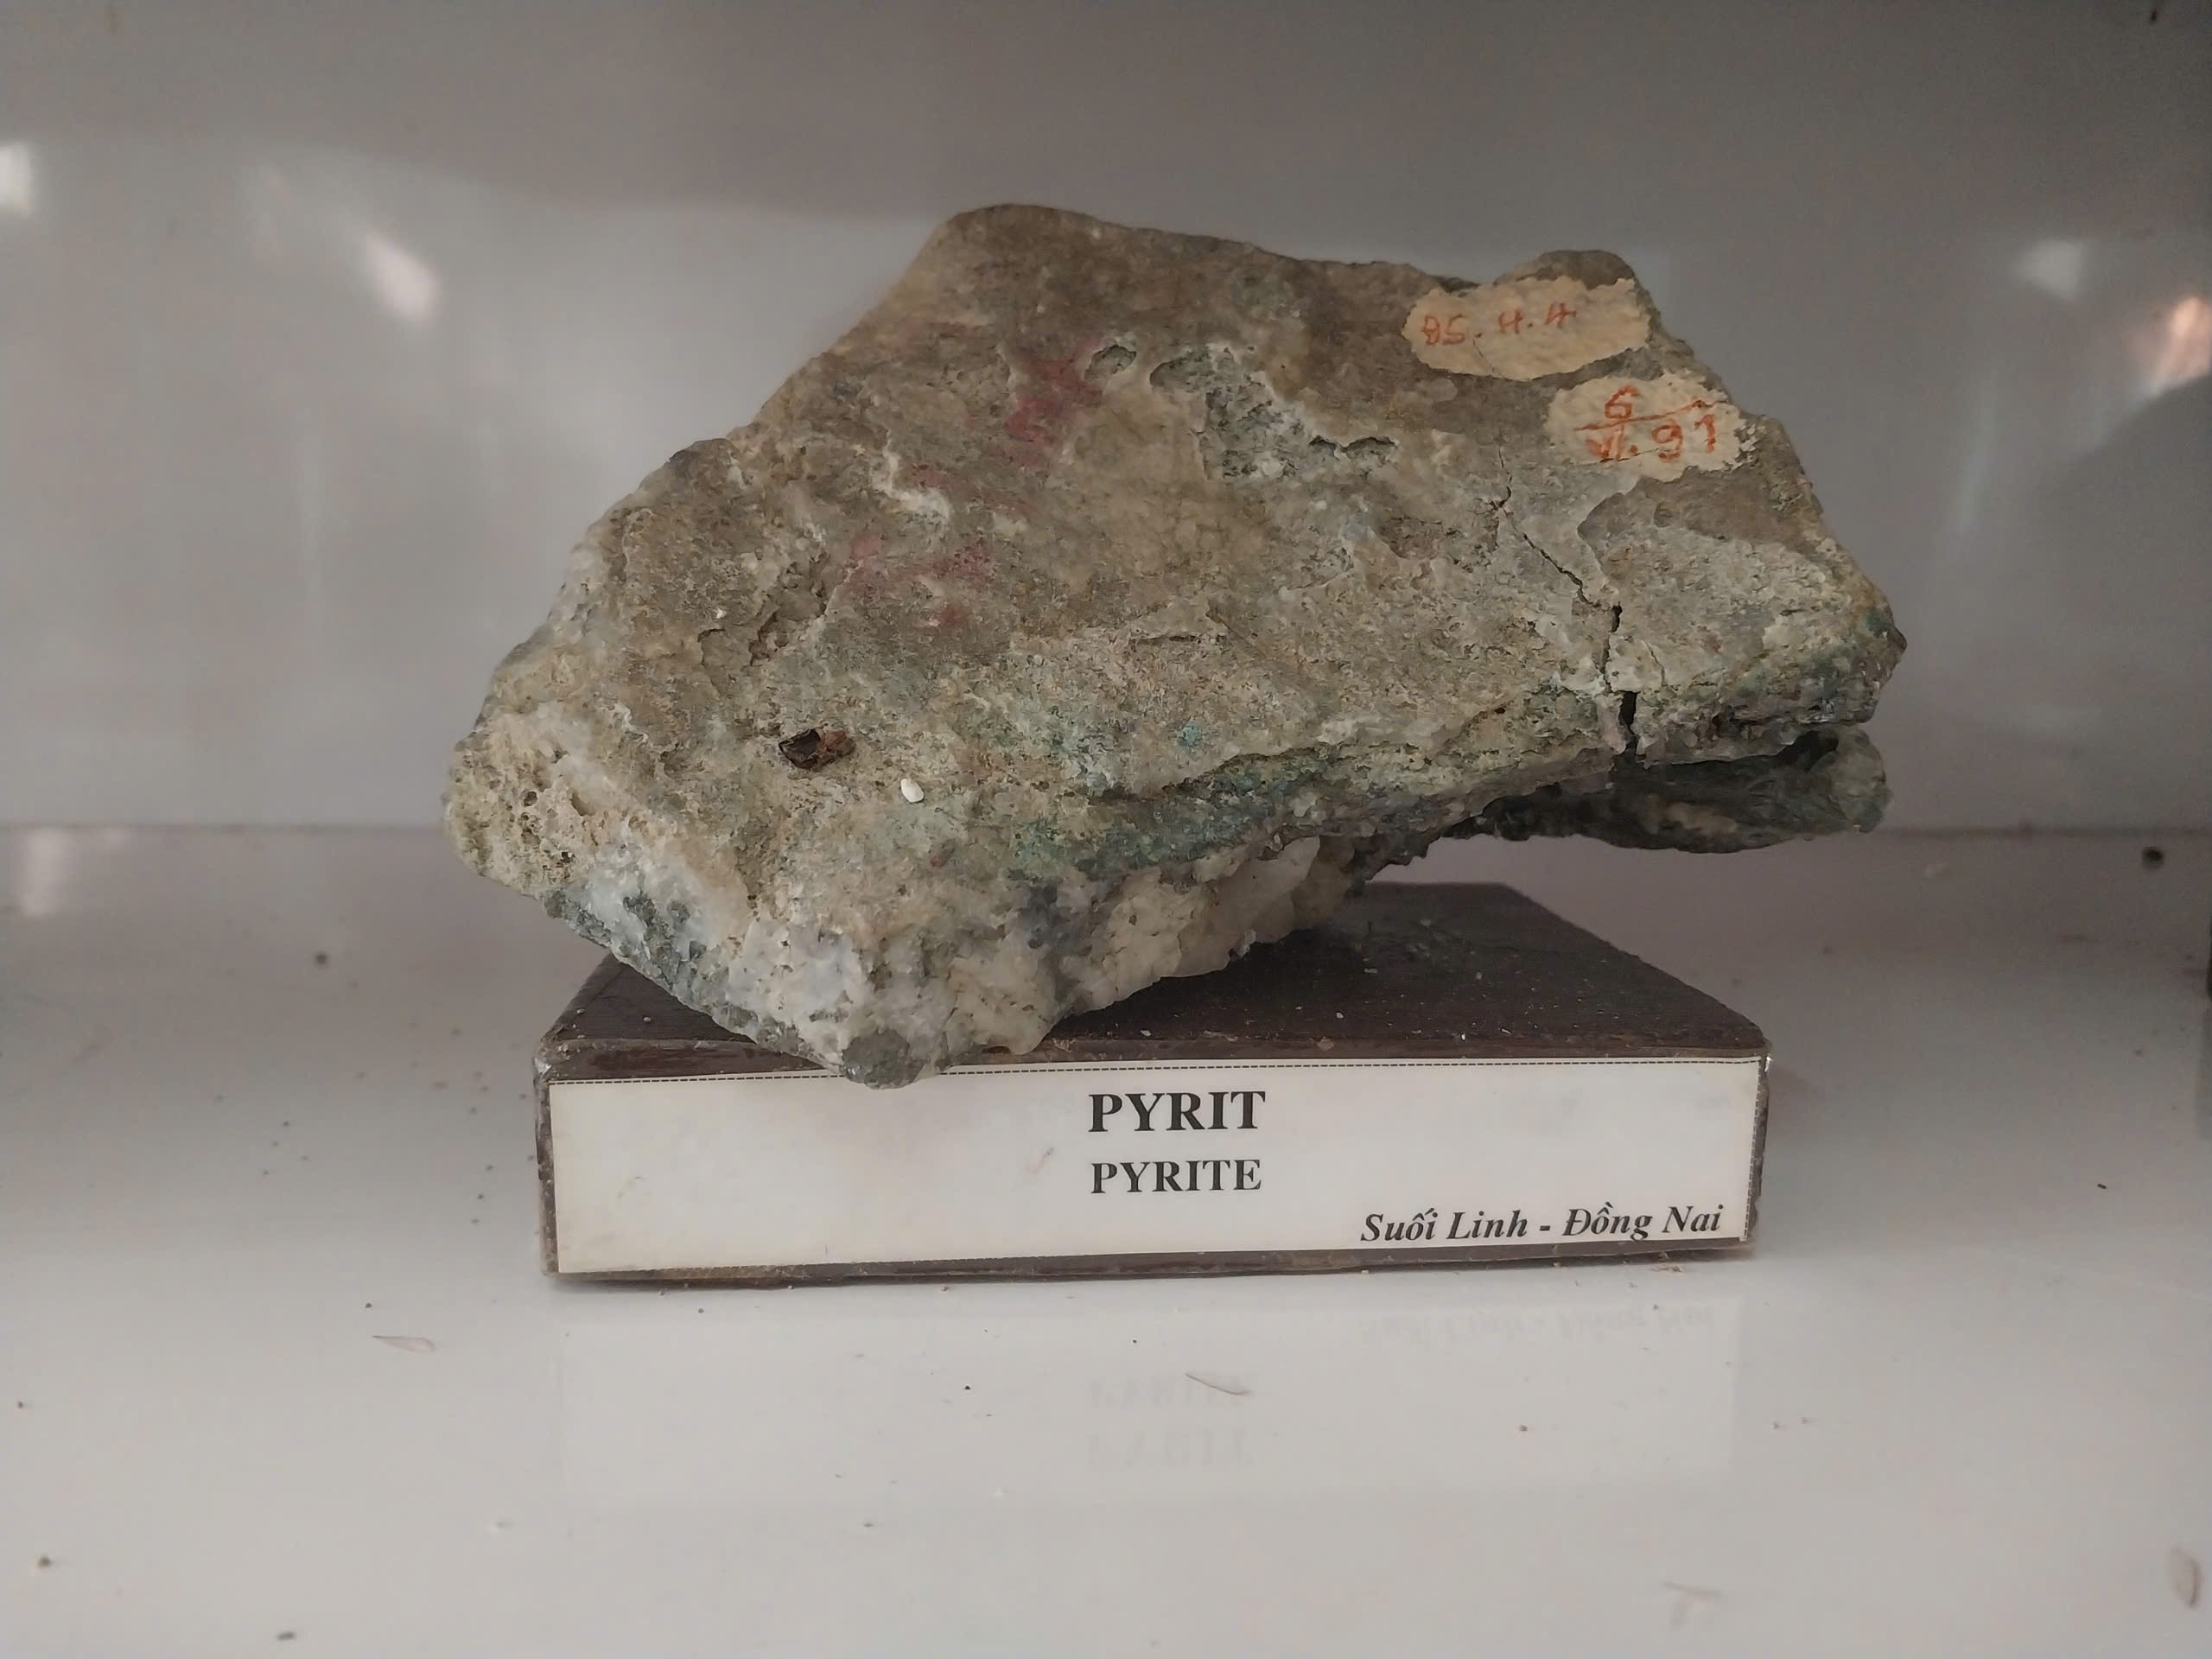
\includegraphics[width=0.7\textwidth]{graphics/pyrite.png}
\caption{Pyrite specimen showing characteristic metallic luster}
\label{fig:pyrite}
\end{figure}

\textit{Talc:} A soft silicate mineral used in cosmetics, paper, paint, and ceramic industries due to its lubricating properties and chemical inertness.

\textit{Asbestos:} Fibrous silicate minerals with heat-resistant properties, though their use is now restricted due to health concerns.

\textit{Kaolin:} A fine clay mineral used in ceramics, paper production, and as a filler in various industrial applications.

\textbf{Agricultural Minerals}
\textit{Apatite:} Phosphate mineral essential for fertilizer production and chemical industries. Vietnam has significant apatite deposits that support the country's agricultural sector through phosphate fertilizer production.

\textit{Phosphorite:} Sedimentary rock containing phosphate minerals, primarily used for fertilizer production.

\subsection{Construction Materials}

Construction materials encompass naturally occurring substances utilized in building and infrastructure development. These materials form the foundation of human civilization's architectural achievements and continue to play crucial roles in modern construction practices.

\textbf{Stone Materials}
\textit{Limestone:} Sedimentary rock composed primarily of calcium carbonate, essential for cement production and construction. Vietnam has extensive limestone deposits throughout the country.

\textit{Marble:} Metamorphosed limestone prized for decorative applications and high-end construction projects. Vietnamese marble is known for its quality and diverse colors.

\textit{Granite:} Igneous rock valued for its durability and aesthetic appeal in construction and monuments. Vietnam has significant granite quarries producing various colors and textures.

\begin{figure}[H]
\centering
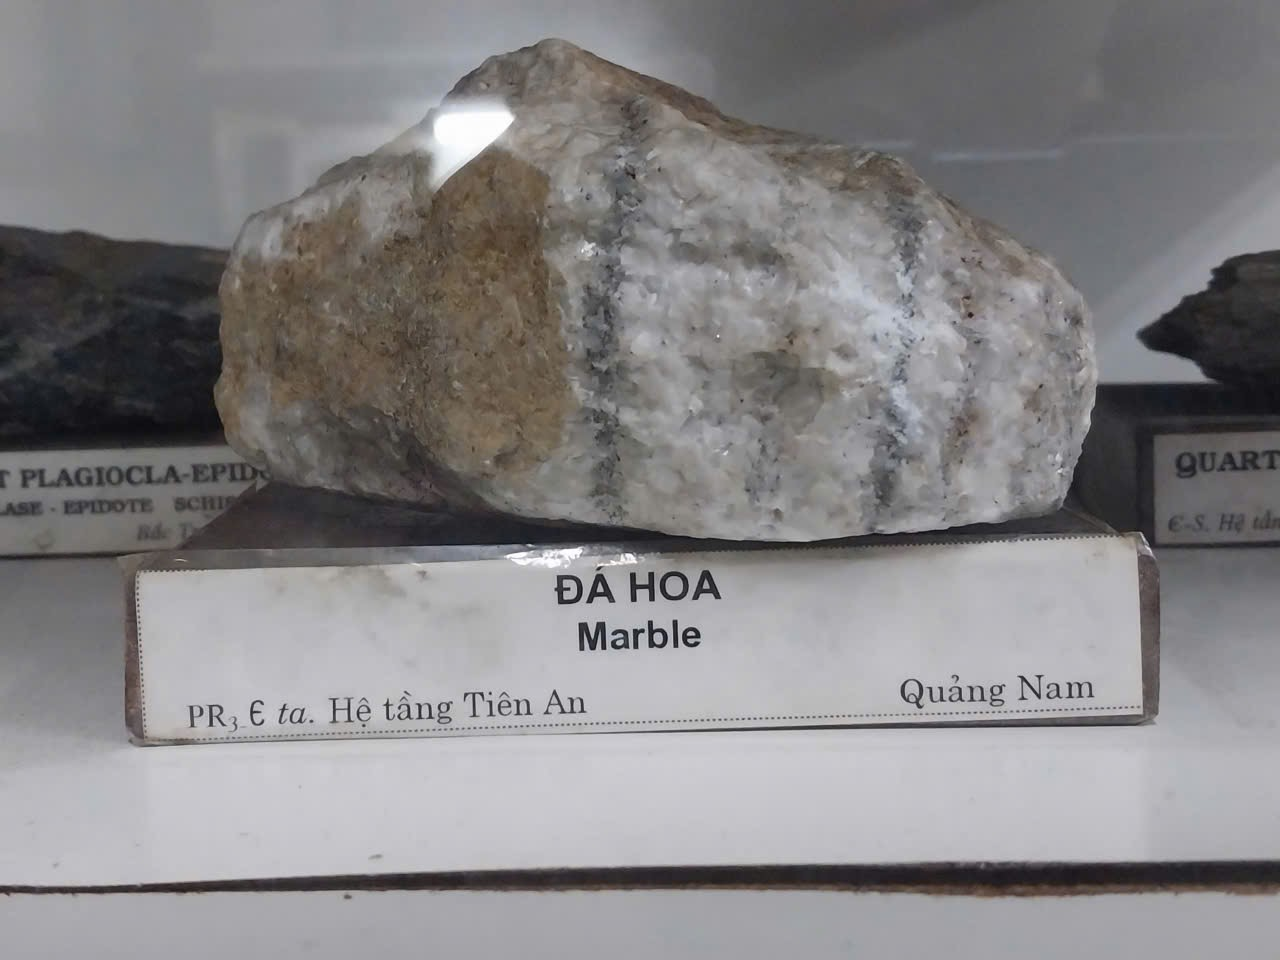
\includegraphics[width=0.7\textwidth]{graphics/stone_materials.png}
\caption{Marble sample}
\label{fig:stone_materials}
\end{figure}

\textbf{Clay and Ceramic Materials}
\textit{Clay:} Fine-grained sedimentary material essential for brick, tile, and ceramic production. Vietnam has abundant clay deposits suitable for various ceramic applications.

\textit{Kaolin:} High-quality white clay used in fine ceramics and porcelain production.


\textbf{Aggregate Materials}
\textit{Sand:} Essential component for concrete production and construction applications. Vietnam has both river sand and marine sand resources.

\textit{Gravel:} Coarse aggregate material used in concrete and road construction.

\textit{Crushed Stone:} Processed stone aggregate for various construction applications.

\begin{figure}[H]
    \centering
    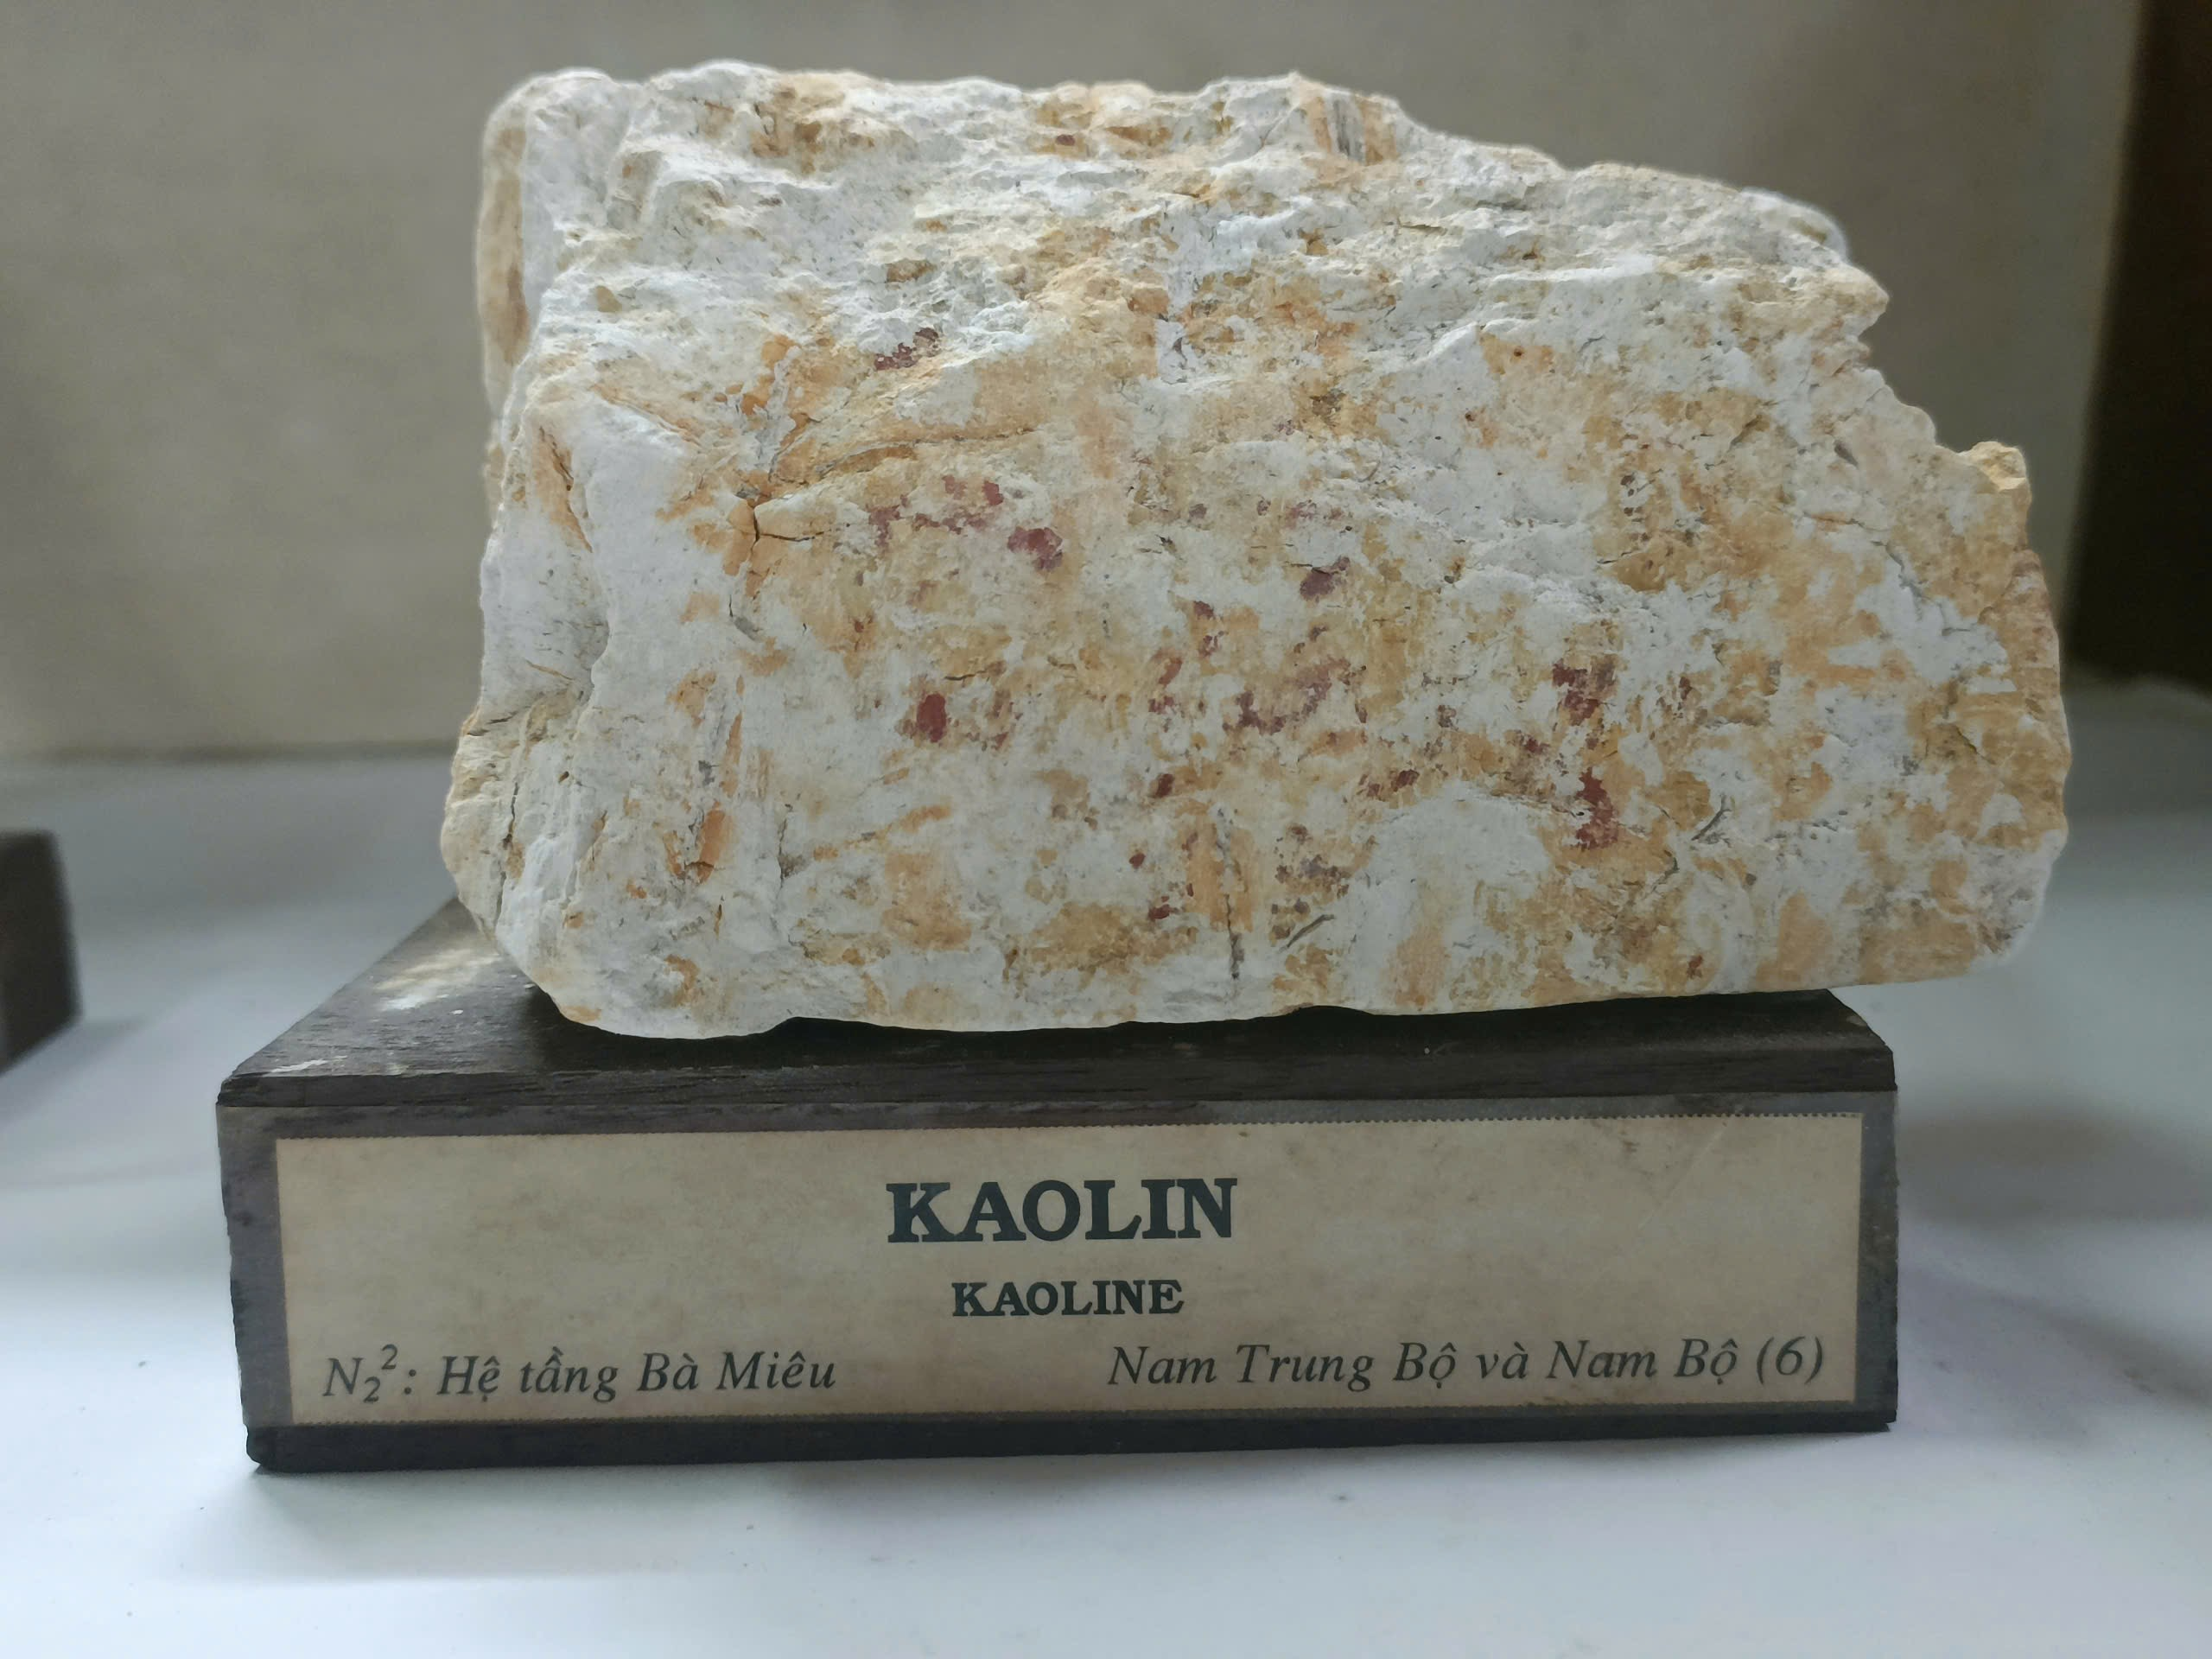
\includegraphics[width=0.7\textwidth]{graphics/kaolin_clay.png}
    \caption{Kaolin clay sample showing characteristic white coloration and fine texture}
    \label{fig:kaolin_clay}
\end{figure}

\subsection{Gemstones and Semi-Precious Stones}

Vietnam possesses notable gemstone deposits with both aesthetic and economic value.

\textbf{Quartz Varieties}
\textit{Amethyst:} A purple variety of quartz that is highly prized for jewelry and decorative purposes. The purple color comes from trace amounts of iron and aluminum impurities. Amethyst is found in various locations throughout Vietnam and is considered one of the most valuable quartz varieties.

\begin{figure}[H]
\centering
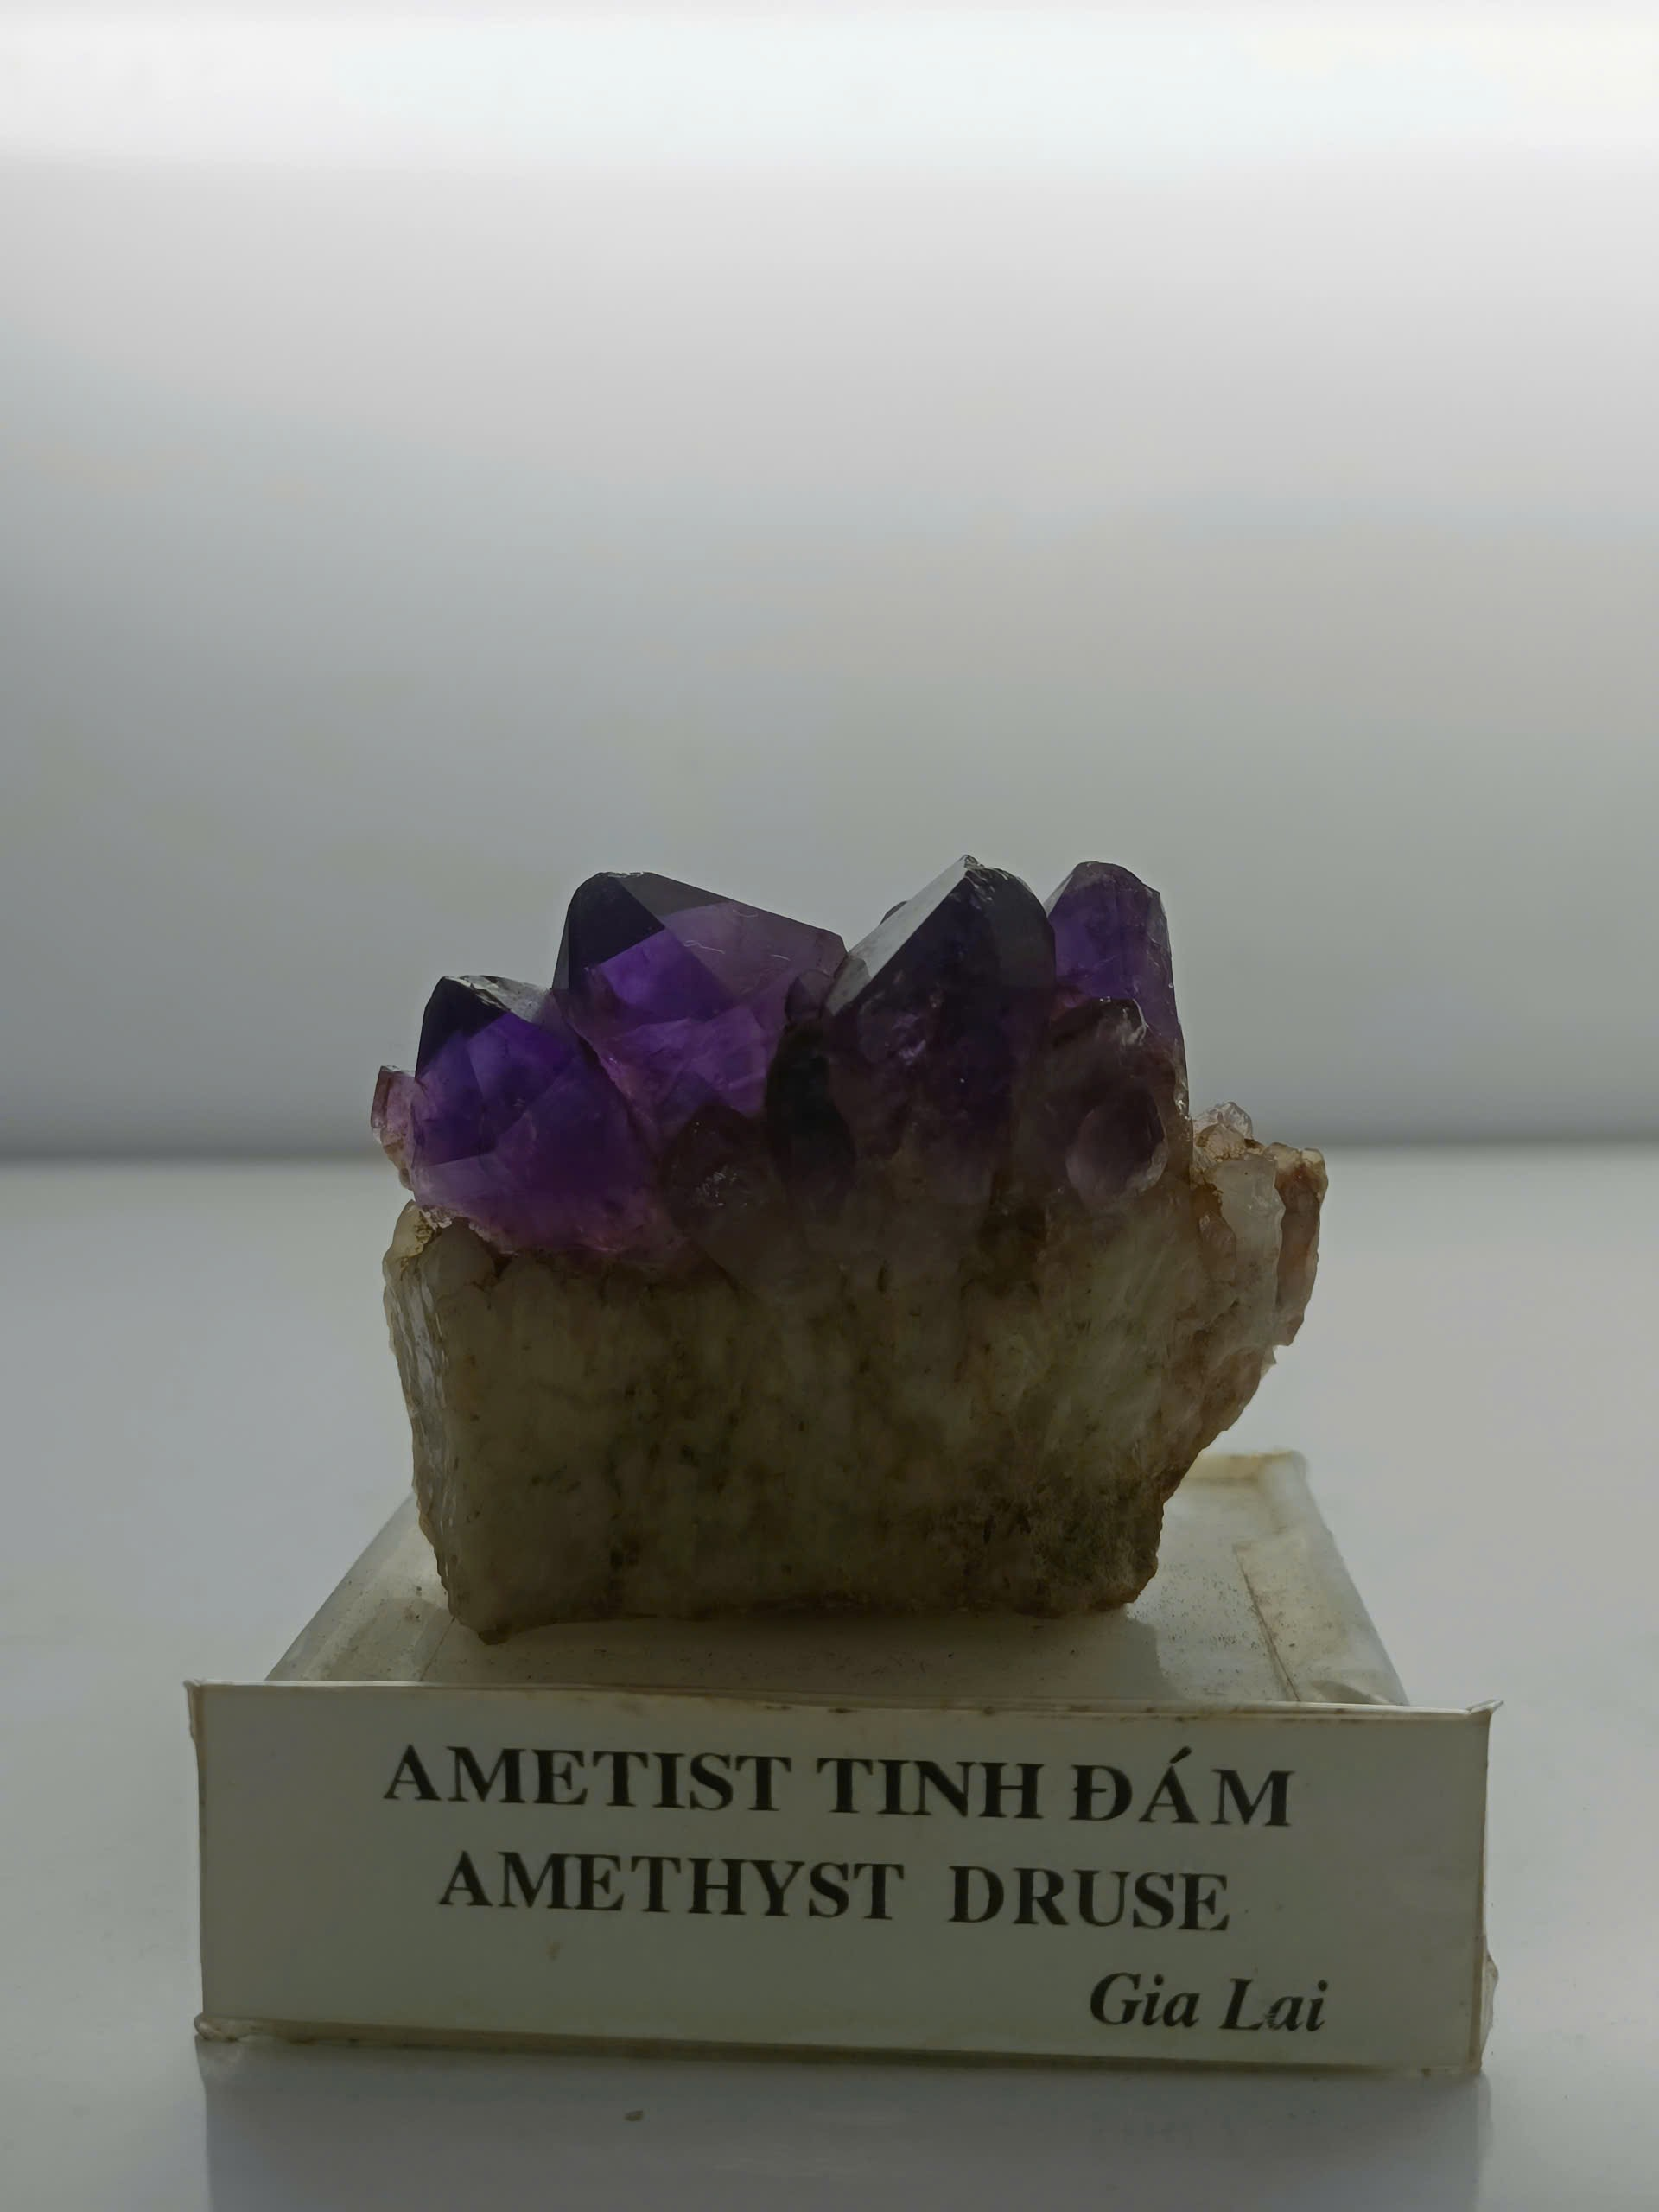
\includegraphics[width=0.7\textwidth]{graphics/amethyst.png}
\caption{Amethyst sample showing characteristic purple coloration}
\label{fig:amethyst}
\end{figure}

\textit{Chalcedony:} A cryptocrystalline form of silica composed of tiny quartz crystals. It typically has a waxy or glassy luster and comes in various colors including white, gray, blue, and brown. Chalcedony is commonly used in jewelry and decorative objects.



\textit{Quartz Crystals:} Clear crystalline quartz formations that are hexagonal in shape with pyramid-shaped termination points. These are used in both jewelry and industrial applications.



\textbf{Precious Gemstones}
\textit{Ruby:} A red variety of the mineral corundum, colored by trace amounts of chromium. Ruby is one of the most valuable gemstones and is highly prized for jewelry. Vietnamese rubies are found in marble formations and are known for their quality.

\begin{figure}[H]
\centering
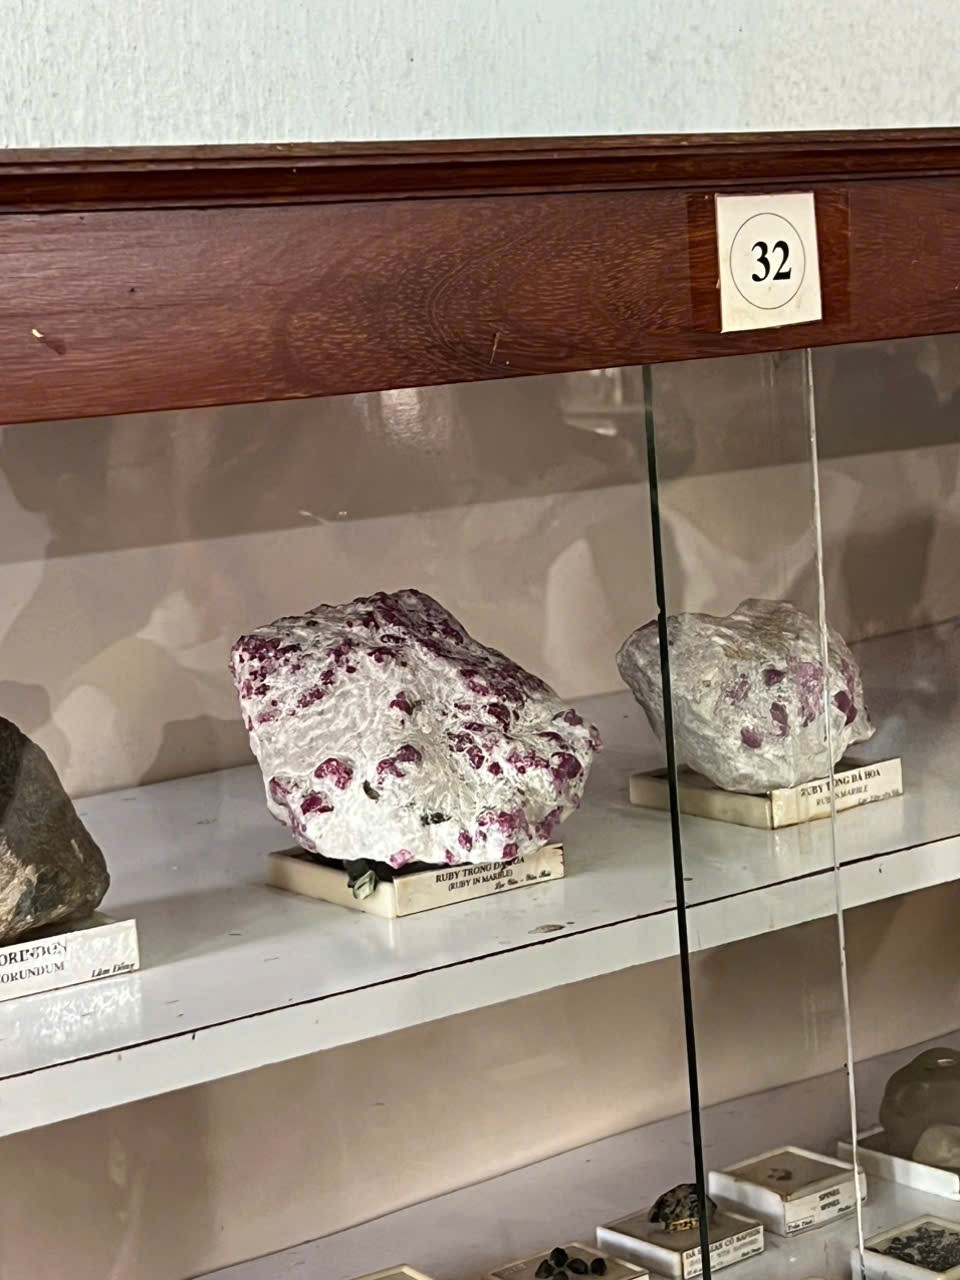
\includegraphics[width=0.7\textwidth]{graphics/ruby.png}
\caption{Ruby samples including ruby in marble matrix}
\label{fig:ruby}
\end{figure}

\textit{Topaz:} A rare silicate mineral with the chemical composition \ce{Al2SiO4(F,OH)2}. While pure topaz is colorless, trace elements can create various colors including blue, golden-brown, and yellow-orange. Topaz is valued for its hardness and brilliance in jewelry applications.

\begin{figure}[H]
\centering
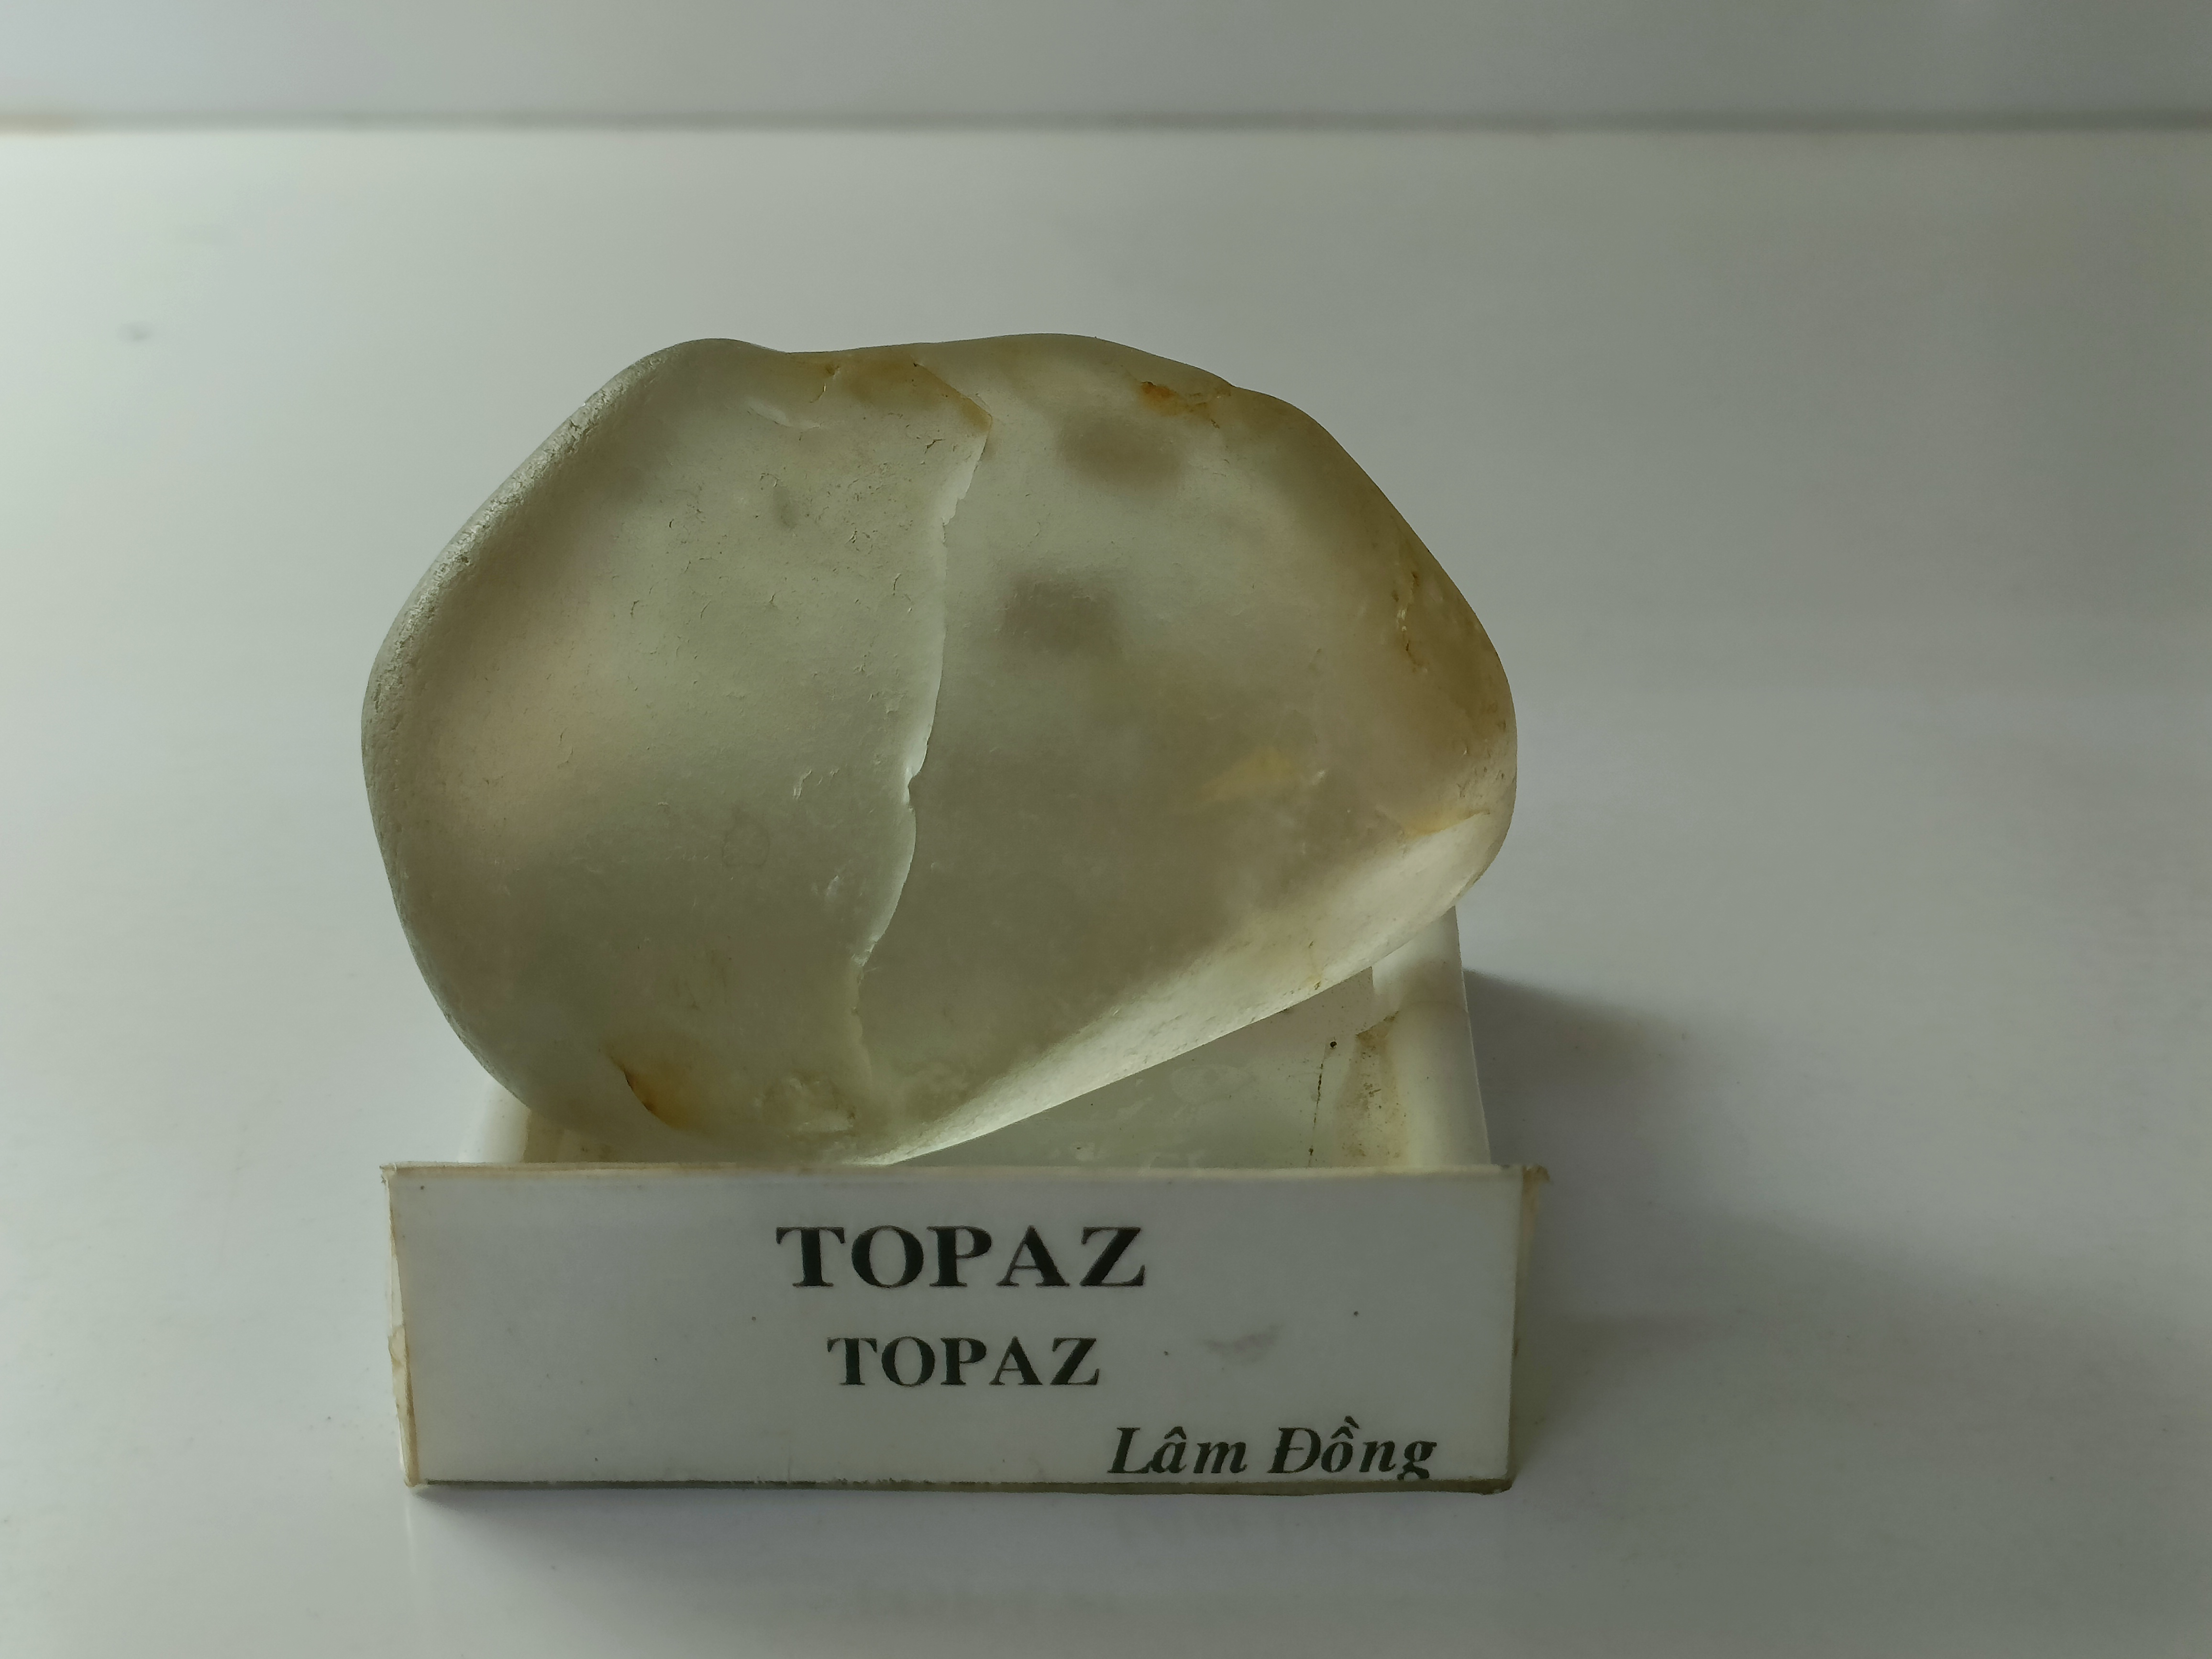
\includegraphics[width=0.7\textwidth]{graphics/topaz.jpg}
\caption{Topaz sample showing characteristic crystal structure}
\label{fig:topaz}
\end{figure}



\subsection{Mineral Water Resources}

Vietnam possesses significant mineral water resources with therapeutic and commercial value.

Natural mineral water is derived from underground sources where water has gradually acquired minerals while flowing through layers of rock over extended periods. Vietnam has numerous mineral water sources with diverse chemical compositions and therapeutic properties.

\textbf{Formation Process}
Groundwater penetrates deep underground, acquiring precious minerals and sometimes heating up in areas with tectonic activity, such as fault lines or historic volcanic zones. This process produces mineral-rich or hot springs that are geologically remarkable and recognized for their health benefits.

\textbf{Vietnamese Sources}
Vietnam has mineral water sources in various regions including Binh Thuan and Ninh Thuan provinces. Notable sources include:
\begin{itemize}
\item \textit{Vinh Hao:} Discovered by the French in 1928 in Vinh Hao, Tuy Phong, Binh Thuan
\item \textit{Van Lam:} Located in the northern regions
\item \textit{Ham Cuong:} Found in central Vietnam
\item \textit{Da Kai:} Another significant source
\end{itemize}

\textbf{Chemical Composition}
Vinh Hao mineral water, due to the perfect geological conditions of the Southeast Truong Son region with numerous interwoven rock layers, has:
\begin{itemize}
\item High concentration of bicarbonate (\ce{HCO3-}) - acts as an antacid to reduce stomach acidity
\item Silicate dissolved in water - beneficial for digestion and nervous system
\item Calcium - prevents osteoporosis
\item Magnesium - strengthens immunity, improves heart function, and regulates blood pressure
\end{itemize}



\subsection{Geological Heritage}

Geological heritage represents a collection of geological resources with exceptional scientific, educational, artistic, and economic significance.

\textbf{Definition and Components}
Geological heritage refers to specific locations or landscapes on Earth that preserve evidence of the planet's formation and evolution, as well as the evolutionary history of life. Components include:
\begin{itemize}
\item Geomorphological landscapes
\item Paleontological sites and fossils
\item Extinct or active volcanic craters
\item Caves and river canyons
\item Natural lakes and waterfalls
\item Rock and ore exposures
\item Geological formations recording special events
\item Sites where geological processes can be observed
\end{itemize}

\textbf{Importance and Conservation}
Geological heritage sites have significant scientific, aesthetic, and historical importance, as well as tourism potential. Like other types of heritage, geological heritage is a finite resource that must be maintained, developed, and used sustainably.

\textbf{Vietnamese Context}
Vietnam's geological heritage includes diverse formations representing different geological periods and processes, from ancient Precambrian rocks to recent volcanic activity, providing valuable insights into Earth's history and geological evolution.